% #############################################################################
% This is the MAIN DOCUMENT of the Thesis MSc TEMPLATE.
% The content for the Thesis MSc is to be written in separate documents
% located in the folder ./Chapters
%         Aknowledgments.tex
%         Abstract.tex
%         KeyWords.tex
%         Resumo.tex
%         PalavrasChave.tex
%         Acronyms.tex
%         Front_Cover.tex
%         Chapter_1.tex ....Chapter_2 .....
%         ApendixA.tex ... ApendixB.tex...
% -----------------------------------------------------------------------------
% The class "istulthesis" is based on the standard LaTeX 'report' class.
% It can be used for Instituto Superior Tecnico thesis, as it follows the 
% regulations published by the Scientific Council of IST.
% The class defines the document style. 
% IST requires the thesis to be written in Arial or similar. 
% Two arguments in '\documentclass' allow you to define the thesis font: 
% 'Helvetica' and 'AvantGarde', which transforms 
% the default LaTeX font into Helvetica or AvantGarde, respectively.
% #############################################################################
% The document is automatically set for english or portuguese by just selecting
% the MAIN LANGUAGE in file 'Thesis-MSc-Preamble_commands.tex' 
% #############################################################################
% Thesis-MSc
% Version 2.0, August 2018
% BY: Rui Santos Cruz, rui.s.cruz@tecnico.ulisboa.pt
% #############################################################################
% !TEX root = ./main.tex
% -----------------------------------------------------------------------------
%
\documentclass[defaultstyle,10pt,Helvetica]{istulthesis}
%
% -----------------------------------------------------------------------------
% The Preamble document contains all the necessary Packages for typesetting
% Modify it to suit your needs
% -----------------------------------------------------------------------------
% #############################################################################
% Preamble for Thesis-MSc in English or Portuguese
% Required Packages and commands
% --> Please Choose the MAIN LANGUAGE for the Thesis in package BABEL (below)
% !TEX root = ./main.tex
% #############################################################################
% Thesis-MSc
% Version 2.0, August 2018
% BY: Rui Santos Cruz, rui.s.cruz@tecnico.ulisboa.pt
% #############################################################################
%
% -----------------------------------------------------------------------------
% PACKAGES ucs, utf8x, babel, iflang:
% -----------------------------------------------------------------------------
% The 'ucs' package provides support for using UTF-8 in LaTeX documents. 
% However in most situations it is not required.
\usepackage{ucs}
% The 'utf8x' package contains support for using UTF-8 as input encoding. 
\usepackage[utf8x]{inputenc}
% The 'babel' package may correct some hyphenation issues of LaTeX. 
% Select your MAIN LANGUAGE for the Thesis with the 'main=' option.
\usepackage[main=english,portuguese]{babel}
% The 'iflang' package is used to help determine the language being used. 
\usepackage{iflang}


%% ______________________________ RAFA ______________________________________
%% ______________________________ RAFA ______________________________________



%ALLOW METACODE CREATION
% \usepackage{algorithm}
% \usepackage[noend]{algpseudocode}




%% ______________________________ RAFA ______________________________________
%% ______________________________ RAFA ______________________________________


% -----------------------------------------------------------------------------
% PACKAGE scrbase:
% -----------------------------------------------------------------------------
% The 'scrbase' package is used to help redefining document structure.
\usepackage{scrbase}
% -----------------------------------------------------------------------------
% PACKAGE mathtools, amsmath, amsthm, amssymb, amsfonts, nicefrac:
% -----------------------------------------------------------------------------
% These packages are typically required. 
% Among many other things they add the possibility to put symbols in bold
% by using \boldsymbol (not \mathbf); defines additional fonts and symbols;
% adds the \eqref command for citing equations.
\usepackage{mathtools, amsmath, amsthm, amssymb, amsfonts}
\usepackage{nicefrac}
%
% -----------------------------------------------------------------------------
% PACKAGE tikz:
% -----------------------------------------------------------------------------
% Tikz  for creating graphics programmatically.
\usepackage{tikz}
\usetikzlibrary{shapes.geometric, arrows, positioning}
% -----------------------------------------------------------------------------
% PACKAGES array, booktabs, multirow, colortbl, ctable, spreadtab:
% -----------------------------------------------------------------------------
% These packages are most usefull for advanced tables. 
% 'multirow' allows to join rows throuhg the command \multirow which works
% similarly with the command \multicolumn.
% The 'colortbl' package allows to color the table (foreground and background)
% The 'ctable' package provides commands to easily typeset centered or left or
% right aligned tables.
% The package 'booktabs' provide some additional commands to enhance
% the quality of tables
% The 'longtable' package is only required when tables extend beyond the length
% of one page, which typically does not happen and should be avoided
\usepackage{array}
\usepackage{booktabs}
\usepackage{multirow}
\usepackage{colortbl}
\usepackage{ctable}
\usepackage{spreadtab}
\usepackage{longtable}
%
% -----------------------------------------------------------------------------
% PACKAGES graphicx, subfigure:
% -----------------------------------------------------------------------------
% The package 'graphicx' supports formats PNG and JPG.
% Package 'subfigure' allows to place figures within figures with own caption. 
% For each of the subfigures use the command \subfigure.
\usepackage{graphicx}
\usepackage[hang,small,bf,tight]{subfigure}
%
% -----------------------------------------------------------------------------
% PACKAGE caption:
% -----------------------------------------------------------------------------
% The 'caption' package offers customization of captions in floating 
% environments such figure and table
% \usepackage[hang,small,bf]{caption}
\usepackage[format=hang,labelfont=bf,font=small]{caption} 
% the following customization adds vertical space between caption and the table
\captionsetup[table]{skip=10pt}
%
% -----------------------------------------------------------------------------
% PACKAGE algorithmic, algorithm, algorithm2e:
% -----------------------------------------------------------------------------
% These packages are required if you need to describe an algorithm.
% The preference is for using 'algorithm2e'
%\usepackage{algorithmic}
%\usepackage[chapter]{algorithm}
\usepackage[ruled,vlined,algochapter,norelsize,\languagename]{algorithm2e}
%
% -----------------------------------------------------------------------------
% PACKAGE listings
% -----------------------------------------------------------------------------
% These packages are required if you need to list code snippets.
\usepackage{listings}
% Nicely syntax highlighted m-code in LaTeX documents with stylefile mcode.sty
% http://www.mathworks.com/matlabcentral/fileexchange/8015-m-code-latex-package
\usepackage[numbered]{./tables_and_code/mcode}
%
% -----------------------------------------------------------------------------
% Re-define listings captions and titles based on language.
\newcaptionname{portuguese}{\lstlistingname}{Listagem} % Listings CAPTIONS
\newcaptionname{portuguese}{\lstlistlistingname}{Listagens} % LIST of LISTINGS
%
% -----------------------------------------------------------------------------
% PACKAGE csquotes
% -----------------------------------------------------------------------------
% Quotation helper package
\usepackage{csquotes}
%
% -----------------------------------------------------------------------------
% PACKAGE todonotes
% -----------------------------------------------------------------------------
% Create TODO Notes in text
% The notes can be made invisible by just using the 'disable' option:
\usepackage[textwidth=2cm, textsize=small]{todonotes}
%\usepackage[textwidth=2cm, textsize=small, disable]{todonotes}
\setlength{\marginparwidth}{2cm}
%
% -----------------------------------------------------------------------------
% PACKAGE changes
% -----------------------------------------------------------------------------
% Track changes in document (changes in pdf preview).
%% Use "final" option to make all tracking markups invisible.
%\usepackage[authormarkup=superscript,authormarkuptext=id,markup=underlined,ulem={ULforem,normalbf},final]{changes}
\usepackage[authormarkup=superscript,authormarkuptext=id,markup=underlined,ulem={ULforem,normalbf}]{changes}
% commands:
% \added[id=xx]{text}
% \deleted[id=xx]{text}
% \replaced[id=xx]{deleted text}{added text}
% -----------------------------------------------------------------------------
% PACKAGES xcolor, color
% -----------------------------------------------------------------------------
% These packages are required for list code snippets.
\usepackage{xcolor}
\usepackage{color}
% The following special color definitions are used in the IST Thesis
\definecolor{forestgreen}{RGB}{34,139,34}
\definecolor{orangered}{RGB}{239,134,64}
\definecolor{lightred}{rgb}{1,0.4,0.5}
\definecolor{orange}{rgb}{1,0.45,0.13}	
\definecolor{darkblue}{rgb}{0.0,0.0,0.6}
\definecolor{lightblue}{rgb}{0.1,0.57,0.7}
\definecolor{gray}{rgb}{0.4,0.4,0.4}
\definecolor{lightgray}{rgb}{0.95, 0.95, 0.95}
\definecolor{darkgray}{rgb}{0.4, 0.4, 0.4}
\definecolor{editorGray}{rgb}{0.95, 0.95, 0.95}
\definecolor{editorOcher}{rgb}{1, 0.5, 0} % #FF7F00 -> rgb(239, 169, 0)
\definecolor{chaptergrey}{rgb}{0.6,0.6,0.6}
\definecolor{editorGreen}{rgb}{0, 0.5, 0} % #007C00 -> rgb(0, 124, 0)
\definecolor{olive}{rgb}{0.17,0.59,0.20}
\definecolor{brown}{rgb}{0.69,0.31,0.31}
\definecolor{purple}{rgb}{0.38,0.18,0.81}
%
% -----------------------------------------------------------------------------
% PACKAGE setspace:
% ----------------------------------------------------------------------------
% Provides support for setting the spacing between lines in a document. 
% Package options include single spacing, one half spacing, and double spacing. 
% Alternatively the spacing can be changed as required with:
% \singlespacing, \onehalfspacing, and \doublespacing commands
\usepackage{setspace}
%
% -----------------------------------------------------------------------------
% PACKAGE paralist
% -----------------------------------------------------------------------------
% This package provides the 'inparaenum' environment for inline lists
\usepackage{paralist}
% usage:
% \begin{inparaenum}[(a)]
% \item bla
% \item bla, bla
% \end{inparaenum}
% -----------------------------------------------------------------------------
% PACKAGE cite:
% -----------------------------------------------------------------------------
% The 'cite' package will result in citation numbers being automatically
% sorted and properly "ranged". i.e.,
% [1], [2], [5]--[7], [9]
\usepackage{cite}
%
% -----------------------------------------------------------------------------
% PACKAGE acronym:
% -----------------------------------------------------------------------------
% The package 'acronym' garantees that all acronyms definitions are 
% given at the first usage. 
% IMPORTANT: do not use acronyms in titles/captions; otherwise the definition 
% will appear on the table of contents.
\usepackage[printonlyused]{acronym}
%
% -----------------------------------------------------------------------------
% PACKAGE hyperref
% -----------------------------------------------------------------------------
% Set links for references and citations in document
\usepackage{hyperref}
% pre-configuration of hyperref
\hypersetup{ colorlinks=true,
             citecolor=cyan,
             linkcolor=darkgray,
             urlcolor=teal,
             breaklinks=true,
             bookmarksnumbered=true,
             bookmarksopen=true,
             pdftitle=\@title, % THESIS TITLE
             pdfauthor=\@author,  % YOUR NAME
             pdfcreator=\@author,   % YOUR NAME
}
%
% -----------------------------------------------------------------------------
% PACKAGE url:
% -----------------------------------------------------------------------------
% Provides better support for handling and breaking URLs.
\usepackage{url} 
%
% -----------------------------------------------------------------------------
% PACKAGE Cleveref:
% -----------------------------------------------------------------------------
% Clever Referencing of document parts
% Note: portuguese is supported through "brazilian" option
\usepackage[\IfLanguageName{english}{english}{brazilian}]{cleveref}
%
% -----------------------------------------------------------------------------
% PACKAGE enumitem:
% -----------------------------------------------------------------------------
%For enhanced enumeration of lists
%\usepackage{enumitem}
\usepackage[shortlabels]{enumitem}
\setlist[description]{leftmargin=\parindent,labelindent=\parindent,itemsep=1pt,parsep=0pt,topsep=0pt}
%
% #############################################################################
% GLOBAL FORMATTING OF THE THESIS DOCUMENT before using FANCY stuff
% Set paragraph counter to alphanumeric mode
\renewcommand{\theparagraph}{\Alph{paragraph}~--}
\hoffset 0in
\voffset 0in
\oddsidemargin 0 cm
\evensidemargin 0 cm
\marginparsep 0in
\topmargin -0.25cm
\textwidth 16 cm
\textheight 22.4 cm
\makeatletter
% package indentfirst says \let\@afterindentfalse\@afterindenttrue
% and we revert this modification, reinstating the original definitio
% of \@afterindentfalse
\def\@afterindentfalse{\let\if@afterindent\iffalse}
\makeatother
% -----------------------------------------------------------------------------
% PACKAGE fancyhdr:
% -----------------------------------------------------------------------------
% The fancyhdr macro package allows to customize page headers and footers.
\usepackage{fancyhdr}
\pagestyle{fancy}
\renewcommand{\chaptermark}[1]{\markboth{\thechapter.\ #1}{}}
\renewcommand{\sectionmark}[1]{\markright{\thesection\ #1}}
\fancyhead{}
\renewcommand{\headrulewidth}{0.0pt}
\renewcommand{\footrulewidth}{0.0pt}
\addtolength{\headheight}{2pt} % make space for the rule
\fancypagestyle{plain}{%
   \fancyhead{} % get rid of headers
   \renewcommand{\headrulewidth}{0pt} % and the line
   \renewcommand{\footrulewidth}{0pt}
}
\fancypagestyle{blank}{%
   \fancyhf{} % get rid of headers and footers
   \renewcommand{\headrulewidth}{0pt} % and the line
   \renewcommand{\footrulewidth}{0pt}
}
\fancypagestyle{abstract}{%
   \fancyhead{}
   \renewcommand{\headrulewidth}{0pt}
   \renewcommand{\footrulewidth}{0.0pt}
}
\fancypagestyle{document}{%
	\fancyhead{}
	\renewcommand{\headrulewidth}{0.5pt}
	\renewcommand{\footrulewidth}{0.5pt}
	\addtolength{\headheight}{2pt} % make space for the rule
}
\setcounter{secnumdepth} {5}
\setcounter{tocdepth} {5}
\renewcommand{\thesubsubsection}{\thesubsection.\Alph{subsubsection}}
\renewcommand{\subfigtopskip}{0.3 cm}
\renewcommand{\subfigbottomskip}{0.2 cm}
\renewcommand{\subfigcapskip}{0.3 cm}
\renewcommand{\subfigcapmargin}{0.2 cm}
%
% -----------------------------------------------------------------------------
% PACKAGE minitoc:
% -----------------------------------------------------------------------------
% Package 'minitoc' creates a mini-table of contents (a “minitoc”) at 
% the beginning of each chapter of a document.
% This packages are required for the \fancychapter configuration
\usepackage{minitoc}
\setcounter{minitocdepth}{1}
\setlength{\mtcindent}{24pt}
\renewcommand{\mtcfont}{\small\rm}
\renewcommand{\mtcSfont}{\small\bf}
\renewcommand*{\kernafterminitoc}{\kern0.\baselineskip\kern0.ex}
\mtcselectlanguage{\languagename} 
% Now prepare the MINITOC
\def\boxedverbatim{%
  \def\verbatim@processline{%
    {\setbox0=\hbox{\the\verbatim@line}%
    \hsize=\wd0 \the\verbatim@line\par}}%
  \@minipagetrue%%%DPC%%%
  \@tempswatrue%%%DPC%%%
  \setbox0=\vbox\bgroup\vspace*{0.2cm}\footnotesize\verbatim
}
\def\endboxedverbatim{%
  \endverbatim
  \unskip\setbox0=\lastbox %%%DPC%%%
  \hspace*{0.2cm}
  \vspace*{-0.2cm}
  \egroup
  \fbox{\box0}% <<<=== change here for centering,...
}
% Now prepare the CHAPTER Number
\newcommand*{\chapnumfont}{%
%   \usefont{T1}{\@defaultcnfont}{b}{n}\fontsize{100}{130}\selectfont%
  \usefont{T1}{pbk}{b}{n}
  \fontsize{150}{130}
  \selectfont
  \color{chaptergrey}
}
\makeatletter
\def\@makechapterhead#1{%
  \vspace*{50\p@}%
  {\parindent \z@ \raggedright \normalfont
    {\chapnumfont\ifnum \c@secnumdepth >\m@ne
%         \huge\bfseries \@chapapp\space \thechapter
        \raggedleft\bfseries \thechapter
        \par\nobreak
        \vskip 20\p@
    \fi}
    \interlinepenalty\@M
    {\raggedleft\Huge \bfseries #1\par\nobreak}
    \vskip 40\p@
  }}
\makeatother
% Now put it all together as a command \fancychapter
\newcommand{\fancychapter}[1]{\chapter{#1}\vfill\minitoc\pagebreak}
%
% #############################################################################
% ADDITIONAL COMMANDS AND CONFIGURATIONS
% #############################################################################
% This commmand allows to place horizontal lines with a custom width... 
% replaces the standard hline command
\newcommand{\hlinew}[1]{%
  \noalign{\ifnum0=`}\fi\hrule \@height #1 \futurelet
   \reserved@a\@xhline}
%   
% -----------------------------------------------------------------------------
% This command defines some marks... USEFUL FOR TABLES.
\def\Mark#1{\raisebox{0pt}[0pt][0pt]{\textsuperscript{\footnotesize\ensuremath{\ifcase#1\or *\or \dagger\or \ddagger\or%
    \mathsection\or \mathparagraph\or \|\or **\or \dagger\dagger%
    \or \ddagger\ddagger \else\textsuperscript{\expandafter\romannumeral#1}\fi}}}}
%
% -----------------------------------------------------------------------------
% The following configurations are used for LISTINGS of certain languages
\lstdefinestyle{XML} {
	language=XML,
	extendedchars=true, 
	breaklines=true,
	breakatwhitespace=true,
	emph={},
	emphstyle=\color{red},
	basicstyle=\small,
	xleftmargin=17pt,
	columns=fullflexible,
	commentstyle=\color{gray}\upshape,
	morestring=[b][\color{brown}]",
	morecomment=[s]{<?}{?>},
	morecomment=[s][\color{forestgreen}]{<!--}{-->},
	keywordstyle=\color{orangered},
	stringstyle=\ttfamily\color{black},
	% stringstyle=\ttfamily\color{black}\normalfont,
	tagstyle=\color{blue},
	% tagstyle=\color{darkblue}\bf,
	morekeywords={asn,action,addrType,abilityNAT,audioSampleRate,audiChannels,,bandwidth,bitmapSize,bitRate,connection,codecs,concurrentLinks,dependency,duration,frameRate,from,height,ip,id,lang,mimeType,onlineTime,peerMode,port,priority,peerProtocol,property,release,to,tier,type,transactionID,url,uploadBWlevel,version,width},
	otherkeywords={attribute,xmlns,schemaLocation,PresentationType,availabilityStartTime,availabilityEndTime,minimumUpdatePeriod,minBufferTime,UpdateTime},
}
% ----------------------------------------------------------------------------
\lstdefinelanguage{Assembler}{
	morecomment=[l];,
	keywords={ADD,ADDC,SUB,SUBB,CMP,MUL,DIV,MOD,NEG,AND,OR,NOT,XOR,TEST,BIT,SET,EI,EI0,EI1,EI2,EI3,SETC,EDMA,CLR,DI,DI0,DI1,DI2,DI3,CLRC,SHR,SHL,SHRA,SHLA,ROR,ROL,RORC,ROLC,MOV,MOVB,MOVBS,MOVP,MOVL,MOVH,SWAP,PUSH,POP,JZ,JNZ,JN,JNN,JP,JNP,JC,JNC,JV,JNV,JEQ,JNE,JLT,JLE,JGT,JGE,JA,JAE,JB,JBE,JMP,CALL,CALLF,RET,RETF,SWE,RFE,NOP},
	morekeywords={EQU,TABLE,WORD,STRING,PLACE},
} 
% ----------------------------------------------------------------------------
\lstdefinestyle{coloredASM}{
	language=Assembler,
	extendedchars=false,
	breaklines=true,
	tabsize=2,
	numberstyle=\tiny,
	numbers=left,
	breakatwhitespace=true,
	emph={},
	emphstyle=\color{red},
	fontadjust=true,
	basicstyle=\small\ttfamily,
	% basicstyle=\footnotesize\ttfamily,
	columns=fixed,
	xleftmargin=17pt,
	framexleftmargin=17pt,
	framexrightmargin=5pt,
	framexbottommargin=4pt,
	commentstyle=\color{forestgreen}\upshape,
	morestring=[b][\color{brown}]",
	keywordstyle=\color{darkblue},
	stringstyle=\ttfamily\color{black},
	literate={á}{{\'a}}1 {ã}{{\~a}}1 {â}{{\^a}}1 {é}{{\'e}}1 {É}{{\'E}}1 {ê}{{\^e}}1 {õ}{{\~o}}1 {ó}{{\'o}}1 {í}{{\'i}}1 {ç}{{\c{c}}}1 {Ç}{{\c{C}}}1,
}    
% ----------------------------------------------------------------------------
\lstdefinelanguage{CSS}{
	sensitive=true,
	morecomment=[l]{//},
	morecomment=[s]{/*}{*/},
	morestring=[b]',
	morestring=[b]",
	alsoletter={:},
	alsodigit={-},
	keywords={color,background-image:,margin,padding,font,weight,display,position,top,left,right,bottom,list,style,border,size,white,space,min,width, transition:, transform:, transition-property, transition-duration, transition-timing-function}
}
% ----------------------------------------------------------------------------
% JavaScript
\lstdefinelanguage{JavaScript}{
	morecomment=[s]{/*}{*/},
	morecomment=[l]//,
	morestring=[b]",
	morestring=[b]',
	morekeywords={typeof, new, true, false, catch, function, return, null, catch, switch, var, if, in, while, do, else, case, break}
}
% ----------------------------------------------------------------------------
\lstdefinelanguage{HTML5}{
	language=html,
	sensitive=true,	
	alsoletter={<>=-},	
	morecomment=[s]{<!-}{-->},
	tag=[s],
	otherkeywords={
	% General
	>,
	% Standard tags
	<!DOCTYPE,
	</html, <html, <head, <title, </title, <style, </style, <link, </head, <meta, />,
	% body
	</body, <body,
	% Divs
	</div, <div, </div>, 
	% Paragraphs
	</p, <p, </p>,
	% scripts
	</script, <script,
	% More tags...
	<canvas, /canvas>, <svg, <rect, <animateTransform, </rect>, </svg>, <video, <source, <iframe, </iframe>, </video>, <image, </image>, <header, </header, <article, </article},
	ndkeywords={
	% General
	=,
	% HTML attributes
	charset=, src=, id=, width=, height=, style=, type=, rel=, href=,
	% SVG attributes
	fill=, attributeName=, begin=, dur=, from=, to=, poster=, controls=, x=, y=, repeatCount=, xlink:href=,
	% properties
	margin:, padding:, background-image:, border:, top:, left:, position:, width:, height:, margin-top:, margin-bottom:, font-size:, line-height:,
	% CSS3 properties
	transform:, -moz-transform:, -webkit-transform:,
	animation:, -webkit-animation:,
	transition:,  transition-duration:, transition-property:, transition-timing-function:,
	}
}
% ----------------------------------------------------------------------------
\lstdefinestyle{htmlcssjs} {%
	% General design
	backgroundcolor=\color{editorGray},
		fontadjust=true,
	basicstyle=\small\ttfamily,   
	frame=b,
	% line-numbers
	xleftmargin={0.75cm},
	numbers=left,
	stepnumber=1,
	firstnumber=1,
	numberfirstline=true,	
	% Code design
	identifierstyle=\color{black},
	keywordstyle=\color{blue}\bfseries,
	ndkeywordstyle=\color{editorGreen}\bfseries,
	stringstyle=\color{editorOcher}\ttfamily,
	commentstyle=\color{brown}\ttfamily,
	% Code
	language=HTML5,
	alsolanguage=JavaScript,
	alsodigit={.:;},	
	tabsize=2,
	showtabs=false,
	showspaces=false,
	showstringspaces=false,
	extendedchars=true,
	breaklines=true,
	% German umlauts
	literate=%
	{Ö}{{\"O}}1
	{Ä}{{\"A}}1
	{Ü}{{\"U}}1
	{ß}{{\ss}}1
	{ü}{{\"u}}1
	{ä}{{\"a}}1
	{ö}{{\"o}}1
}
% ----------------------------------------------------------------------------
\lstdefinestyle{py} {%
	language=python,
	literate=%
	*{0}{{{\color{lightred}0}}}1
	{1}{{{\color{lightred}1}}}1
	{2}{{{\color{lightred}2}}}1
	{3}{{{\color{lightred}3}}}1
	{4}{{{\color{lightred}4}}}1
	{5}{{{\color{lightred}5}}}1
	{6}{{{\color{lightred}6}}}1
	{7}{{{\color{lightred}7}}}1
	{8}{{{\color{lightred}8}}}1
	{9}{{{\color{lightred}9}}}1,
	basicstyle=\small\ttfamily,
	numbers=left,
	% numberstyle=\tiny,
	% stepnumber=2,
	numbersep=5pt,
	tabsize=4,
	extendedchars=true,
	breaklines=true,
	keywordstyle=\color{blue}\bfseries,
	frame=b,
	commentstyle=\color{brown}\itshape,
	stringstyle=\color{editorOcher}\ttfamily,
	showspaces=false,
	showtabs=false,
	xleftmargin=17pt,
	framexleftmargin=17pt,
	framexrightmargin=5pt,
	framexbottommargin=4pt,
	backgroundcolor=\color{lightgray},
	showstringspaces=false,
}
%
% #############################################################################
% #############################################################################
\begin{document}
%
% Add PDF bookmark 
\pdfbookmark[0]{Titlepage}{Title}
% #############################################################################
% DEFINE THE Front Cover Page of Thesis-MSc
% !TEX root = ./main.tex
% #############################################################################
% Thesis-MSc
% Version 2.0, August 2018
% BY: Rui Santos Cruz, rui.s.cruz@tecnico.ulisboa.pt
% #############################################################################
%
% REQUIRED LOGO:
% The university logo image: arguments correspond to {left}{top} position. 
% IST rules determine the position to be be 2cm from top, left page edge
\univlogo{2cm}{2cm}{./Images/IST_A_RGB_POS}
% OPTIONAL IMAGE:
% The thesis image: arguments are the start position in the page.
% You can change the image for your thesis, replacing the image name:
%\thesislogo{2.5cm}{6cm}{./Images/thesis_logo}
\thesislogo{2.5cm}{6cm}{./Images/tecnico-lisboa}
%
% -----------------------------------------------------------------------------
% REQUIRED: Thesis TITLE
\title{Flight Time and Cost Minimization in Complex Routes}
% OPTIONAL: Thesis SUBTITLE
%\subtitle{This is the Thesis Subtitle if Necessary}
%
% -----------------------------------------------------------------------------
% REQUIRED: Author
% Author full Name
\author{Rafael Alexandre da Silva Marques}
%
% -----------------------------------------------------------------------------
% The official name of the course/degree. Please chose portuguese or english
% un-comment the line corresponding to your degree.
% You can add a degree name using this construct
%
\degree{Masters in Aerospace Engineering}
%
% -----------------------------------------------------------------------------
% REQUIRED: The SUPERVISOR(s) - maximum of two
\supervisor{Prof. Nuno Roma}
%\supervisor{Prof. Luis Russo}
% If no co-Supervisor comment the next line
\othersupervisor{Prof. Prof. Luis Russo}
%
% -----------------------------------------------------------------------------
% REQUIRED: Date of examination
% Insert the Date of the Thesis discussion (format is MONTH and YEAR)
\date{October 2018}
%
% -----------------------------------------------------------------------------
% The following command define the author colors for Tracking Changes in doc
\definechangesauthor[color=forestgreen]{MN}
\definechangesauthor[color=blue]{JO}
\definechangesauthor[color=red]{PT}

% -----------------------------------------------------------------------------
% Place 'false' when delivering the draft version of the thesis.
% The committee members should not be printed for the draft version. 
% Place 'true' after the Examination Committee has accepted the thesis as final
\finalthesis{true}
%\finalthesis{false}
%
% -----------------------------------------------------------------------------
% The members of the Examination Committee
\chairperson{Prof. Name of the Chairperson}
\vogalone{Prof. Name of First Committee Member}
\vogaltwo{Dr. Name of Second Committee Member}
\vogalthree{Eng. Name of Third Committee Member}
%
% -----------------------------------------------------------------------------
% Please DO NOT MODIFY the following lines.
% print the titlepage
\maketitle
\clearpage
\thispagestyle{empty}
% If Printing on DOUBLE SIDED pages, the second page should be white.
\cleardoublepage
%
% -----------------------------------------------------------------------------
% PAGE NUMBERING FOR INDEXING MATTER in ROMAN
\setcounter{page}{1} \pagenumbering{roman}
\baselineskip 18pt % line spacing: -12pt for single spacing
                   %               -18pt for 1 1/2 spacing
                   %               -24pt for double spacing
% -----------------------------------------------------------------------------
% THE ACKNOWLEGMENTS
\pdfbookmark[0]{Acknowledgments}{acknowledgments}
\begin{acknowledgments}
	% #############################################################################
% Agradecimentos / Acknowledgments
% !TEX root = ../main.tex
% #############################################################################

I would like to thank my parents for their friendship, encouragement and caring over all these years, for always being there for me through thick and thin and without whom this project would not be possible. I would also like to thank my grandparents, aunts, uncles and cousins for their understanding and support throughout all these years.

Quisque facilisis erat a dui. Nam malesuada ornare dolor. Cras gravida, diam sit amet rhoncus ornare, erat elit consectetuer erat, id egestas pede nibh eget odio. Proin tincidunt, velit vel porta elementum, magna diam molestie sapien, non aliquet massa pede eu diam. Aliquam iaculis. 

Fusce et ipsum et nulla tristique facilisis. Donec eget sem sit amet ligula viverra gravida. Etiam vehicula urna vel turpis. Suspendisse sagittis ante a urna. Morbi a est quis orci consequat rutrum. Nullam egestas feugiat felis. Integer adipiscing semper ligula. Nunc molestie, nisl sit amet cursus convallis, sapien lectus pretium metus, vitae pretium enim wisi id lectus. 

Donec vestibulum. Etiam vel nibh. Nulla facilisi. Mauris pharetra. Donec augue. Fusce ultrices, neque id dignissim ultrices, tellus mauris dictum elit, vel lacinia enim metus eu nunc.

I would also like to acknowledge my dissertation supervisors Prof. Some Name and Prof. Some Other Name for their insight, support and sharing of knowledge that has made this Thesis possible.

Last but not least, to all my friends and colleagues that helped me grow as a person and were always there for me during the good and bad times in my life. Thank you.

To each and every one of you -- Thank you.
\end{acknowledgments}
%
% -----------------------------------------------------------------------------
% THE ABSTRACT
\pdfbookmark[0]{Abstract}{Abstract}
\begin{abstract}
	% #############################################################################
% Abstract Text
% !TEX root = ../main.tex
% #############################################################################
% use \noindent in firts paragraph

\noindent 

%1) Introduction - find the best route, schedule and set of flights for a multi-city trip.
%2) Overview of related problems - gives an idea on what strategies to follow
%3) Formal Definition of the problem and proposed methods to solve it
%4) Designing and implementation a web application for it
%5) Experimental results - optimization system performance, utility of the proposed problem, and comparison to current state of the art.

Despite the existence of numerous flight search applications, most of them lack the ability to properly address multi-city flight requests. The goal of this work is to develop an application that addresses the problem of finding the best route, schedule and set of flights, for any unconstrained multi-city flight request. 

The considered problem belongs to the class of scheduling and routing problems. In particular, it occurs as a generalization of the Traveling Salesman Problem and its time-dependent variation. Thus, an overview of the methodologies implemented in the resolution of these problems may be useful for the definition of an adequate strategy to the resolution of the considered problem. 

This work proposes a formal definition for the problem under resolution, and denotes it as the Flying Tourist Problem. In order to solve it, this work uses different heuristics and metaheuristics, including the Ant Colony Optimization and the Simulated Annealing. Using these methods, a solution may be constructed in real-time, even for large problem instances.

The methods developed for the resolution of this problem are integrated into a web application, making it publicly available.

The developed system is evaluated using three different criteria: the quality of its optimization system; the utility of the devised problem; and its performance compared to other similar systems. The results are extremely positive, and show that it is possible to
considerable reduce the price and flight duration, even for small problem instances. 

Keywords: Flight search application, Routing and scheduling problem, metaheuristics

%reduce the cost in 15\% on a 5 cities trip, and 33\% on a 10 cities trip.

%The performance of the developed optimization methods is evaluated using a set of benchmark tests, while the utility of the proposed system is determined according to the price savings, when compared to the standard way of solving these type of requests. 
%The results presented in this work are extremely positive, showing that is is possible to reduce the cost in 15\% on a 5 cities trip, and 33\% on a 10 cities trip.
%The results presented in this works are extremely positive, and show that, as the number of cities to visit increases, the proposed system is capable of presenting solutions with a lower flight price and duration, when compared to the standart me


%This problem occurs as a generalization of the Traveling Salesman Problem and thus, an overview of this problem and the methodologies used in its resolution may be useful for the definition of an adequate strategy for the resolution of the considered problem.




% How to Write an Abstract for Your Thesis or Dissertation
% What is an Abstract?
% The abstract is an important component of your thesis. Presented at the beginning of the thesis, it is likely the first substantive description of your work read by an external examiner. You should view it as an opportunity to set accurate expectations.
% The abstract is a summary of the whole thesis. It presents all the major elements of your work in a highly condensed form.
% An abstract often functions, together with the thesis title, as a stand-alone text. Abstracts appear, absent the full text of the thesis, in bibliographic indexes such as PsycInfo. They may also be presented in announcements of the thesis examination. Most readers who encounter your abstract in a bibliographic database or receive an email announcing your research presentation will never retrieve the full text or attend the presentation.
% An abstract is not merely an introduction in the sense of a preface, preamble, or advance organizer that prepares the reader for the thesis. In addition to that function, it must be capable of substituting for the whole thesis when there is insufficient time and space for the full text.
% Size and Structure
% Currently, the maximum sizes for abstracts submitted to Canada's National Archive are 150 words (Masters thesis) and 350 words (Doctoral dissertation).
% To preserve visual coherence, you may wish to limit the abstract for your doctoral dissertation to one double-spaced page, about 280 words.
% The structure of the abstract should mirror the structure of the whole thesis, and should represent all its major elements.
% For example, if your thesis has five chapters (introduction, literature review, methodology, results, conclusion), there should be one or more sentences assigned to summarize each chapter.
% Clearly Specify Your Research Questions
% As in the thesis itself, your research questions are critical in ensuring that the abstract is coherent and logically structured. They form the skeleton to which other elements adhere.
% They should be presented near the beginning of the abstract.
% There is only room for one to three questions. If there are more than three major research questions in your thesis, you should consider restructuring them by reducing some to subsidiary status.
% Don't Forget the Results
% The most common error in abstracts is failure to present results.
% The primary function of your thesis (and by extension your abstract) is not to tell readers what you did, it is to tell them what you discovered. Other information, such as the account of your research methods, is needed mainly to back the claims you make about your results.
% Approximately the last half of the abstract should be dedicated to summarizing and interpreting your results.
\end{abstract}
\begin{keywords}
	% #############################################################################
% English Keywords
% !TEX root = ../main.tex
% #############################################################################
% use \noindent in firts paragraph
%\noindent
Flying Tourist Problem, Traveling Salesman Problem, 
Combinatorial Optimization, Ant Colony Optimization, Simulated 
Annealing, Web Application.
\end{keywords}
\clearpage
\thispagestyle{empty}
%% If Printing on DOUBLE SIDED pages, the second page should be white.
%% Otherwise, comment the following command:
\cleardoublepage
%
% -----------------------------------------------------------------------------
% O RESUMO
\pdfbookmark[0]{Resumo}{Resumo}
\begin{resumo}
	% #############################################################################
% RESUMO em Português
% !TEX root = ../main.tex
% #############################################################################
% use \noindent in firts paragraph
\noindent Pellentesque habitant morbi tristique senectus et netus et malesuada fames ac turpis egestas. Vestibulum tortor quam, feugiat vitae, ultricies eget, tempor sit amet, ante. Donec eu libero sit amet quam egestas semper. Aenean ultricies mi vitae est. Mauris placerat eleifend leo. Quisque sit amet est et sapien ullamcorper pharetra. Vestibulum erat wisi, condimentum sed, commodo vitae, ornare sit amet, wisi. Aenean fermentum, elit eget tincidunt condimentum, eros ipsum rutrum orci, sagittis tempus lacus enim ac dui. Donec non enim in turpis pulvinar facilisis. Ut felis. Aliquam aliquet, est a ullamcorper condimentum, tellus nulla fringilla elit, a iaculis nulla turpis sed wisi. Fusce volutpat. Etiam sodales ante id nunc. Proin ornare dignissim lacus. Nunc porttitor nunc a sem. Sed sollicitudin velit eu magna. Aliquam erat volutpat. Vivamus ornare est non wisi. Proin vel quam. Vivamus egestas. Nunc tempor diam vehicula mauris. Nullam sapien eros, facilisis vel, eleifend non, auctor dapibus, pede.
\end{resumo}
\begin{palavraschave}
	% #############################################################################
% Portuguese Keywords
% !TEX root = ../main.tex
% #############################################################################
% use \noindent in firts paragraph
\noindent 

Flying Tourist Problem, Traveling Salesman Problem, 
Combinatorial Optimization, Ant Colony Optimization, Simulated 
Annealing, Web Application.
\end{palavraschave}
\clearpage
\thispagestyle{empty}
%% If Printing on DOUBLE SIDED pages, the second page should be white.
%% Otherwise, comment the following command:
\cleardoublepage
%
% -----------------------------------------------------------------------------
% This is required for the Fancy Chapters with minitoc
\dominitoc
\dominilof
\dominilot
% -----------------------------------------------------------------------------
% Lists of Contents
\renewcommand{\baselinestretch}{1}
\pdfbookmark[0]{Contents}{toc}
\tableofcontents
%\contentsline{chapter}{References}{\pageref{bib}}
% If Printing on DOUBLE SIDED pages, the second page should be white.
% Otherwise, comment the following command:
\cleardoublepage
% reposition baseline
\renewcommand{\baselinestretch}{1.5}
% -----------------------------------------------------------------------------
% List of Figures
\pdfbookmark[1]{List of Figures}{lof}
\listoffigures
\cleardoublepage
% -----------------------------------------------------------------------------
\begingroup 
    \let\clearpage\relax
    \let\cleardoublepage\relax
    \let\cleardoublepage\relax
% List of Tables
\pdfbookmark[1]{List of Tables}{lot}
\listoftables
% If Printing on DOUBLE SIDED pages, the second page should be white.
% Otherwise, comment the following command:
\let\cleardoublepage\relax
%\cleardoublepage
% -----------------------------------------------------------------------------
% List of Algorithms
% If not used, comments the lines!
% Requires packages algorithmic, algorithm
\pdfbookmark[1]{List of Algorithms}{loa}
\listofalgorithms
% If Printing on DOUBLE SIDED pages, the second page should be white.
\endgroup
% Otherwise, comment the following command:
\cleardoublepage
% -----------------------------------------------------------------------------
% Listings
% If not used, comments the lines!
% Requires packages listings
\pdfbookmark[1]{Listings}{lol}
\lstlistoflistings
\cleardoublepage
% -----------------------------------------------------------------------------
% % List of acronyms
\pdfbookmark[1]{Acronyms}{loac}
\chapter*{\tlangAcronyms}
% #############################################################################
% This is the ACRONYMS Definition
% !TEX root = ../main.tex
% #############################################################################

\begin{acronym}[H.264/SVC]
    \acro{TSP}{Traveling Salesman Problem}
    \acro{ATSP}{Asymmetric Traveling Salesman Problem}
    \acro{TDTSP}{Time-dependent Traveling Salesman Problem}
    \acro{ACO}{Ant Colony Optimization}
    \acro{DTS}{Direct Travel Supplier}
    \acro{API}{Application Programming Interface}
    \acro{FTP}{Flying Tourist Problem}
    \acro{COP}{Combinatorial Optimization Problem}
    \acro{VRP}{Vehicle Routing Problem}
    \acro{ILP}{Integer Linear Programming}
    \acro{BB}{Branch and Bound}
    \acro{SA}{Simulated Annealing}
    \acro{LK}{Lin-Kernighan algorithm}
    \acro{CSA}{Client-side application}        \acro{SSA}{Server-side application}
    \acro{HTTP}{HyperText transfer protocol}
    \acro{AJAX}{Asynchronous JavaScript and XML}
    \acro{URI}{Uniform Resource Identifier}
    \acro{UI}{User Interface}
    \acro{JSON}{JavaScript Object Notation}
    \acro{OS}{Optimization System}
    \acro{DMS}{Data Managemet System}
    \acro{HTML}{HyperText Markup Language}
    \acro{DOM}{Document Object Model}

    \acro{OTA}{Online Travel Agency}
	\acro{AAC}{Advanced Audio Coding}
	\acro{ADTS}{Audio Data Transport Stream}
	\acro{API}{Application Program Interface}
	\acro{AS}{Application Server}
	\acro{AV}{Audio-Visual}
	\acro{AVC}{Advanced Video Coding}
	\acro{BMFF}{Base Media File Format}
	\acro{CC}{Cloud Computing}
	\acro{CDN}{Content Distribution Network}
	\acro{CPU}{Central Processing Unit}
	\acro{DASH}{Dynamic Adaptive Streaming over HTTP}
	\acro{DVD}{Digital Versatile Disk}	
	\acro{ES}{Elementary Stream}
	\acro{ftyp}{File Type}
	\acro{FLV}{Flash Video}
	\acro{GPRS}{General Packet Radio Service}
	\acro{GSM}{Global System for Mobile Communications}
	\acro{H.264/AVC}{Advanced Video Coding}
	\acro{H.264/SVC}{Scalable Video Coding}
	\acro{HD}{High Definition}
	\acro{HDTV}{High Definition Television}
	\acro{HLS}{HTTP Live Streaming}
	\acro{HTTP}{Hypertext Transfer Protocol}
	\acro{IaaS}{Infrastructure as a Service}
	\acro{IETF}{Internet Engineering Task Force}
	\acro{IGMP}{Internet Group Management Protocol}
	\acro{IIS}{Internet Information Services}
	\acro{IMS}{IP Multimedia Subsystem}
	\acro{IP}{Internet Protocol}
	\acro{IPTV}{IP Television}
	\acro{ISP}{Internet Service Provider}
	\acro{IT}{Information Technology}
	\acro{JSVM}{Joint Scalable Video Model}
	\acro{LAN}{Local Area Network}
	\acro{LTE}{Long Term Evolution}
	\acro{MDC}{Multiple Description Coding}
	\acro{MIME}{Multipurpose Internet Mail Extension}
	\acro{MPD}{Media Presentation Description}
	\acro{MPEG}{Moving Picture Expert Group}
	\acro{NAL}{Network Abstraction Layer}
	\acro{NAT}{Network Address Translation}	
	\acro{OS}{Operating System}
	\acro{OSMF}{Open Source Media Framework}
	\acro{P2P}{Peer-to-Peer}
	\acro{PaaS}{Platform as a Service}
	\acro{PES}{Packetized Elementary Streams}
	\acro{QoE}{Quality Of Experience}
	\acro{QoS}{Quality Of Service}
	\acro{QP}{Quantization Parameter}
	\acro{RTCP}{RTP Control Protocol}
	\acro{RTMP}{Real Time Messaging Protocol}
	\acro{RTP}{Real-time Transport Protocol}
	\acro{RTSP}{Real Time Streaming Protocol}
	\acro{SaaS}{Software as a Service}
	\acro{SD}{Standard Definition}
	\acro{SEI}{Supplemental Enhancement Information}
	\acro{SIP}{Selective Inter-layer Prediction}
	\acro{SMS}{Short Message Service}
	\acro{SNR}{Signal-to-Noise Ratio}
	\acro{SVC}{Scalable Video Coding}
	\acro{TCP}{Transport Control Protocol}
	\acro{TS}{Transport Stream}
	\acro{TTL}{Time-to-Live}
	\acro{UDP}{User Datagram Protocol}
	\acro{UI}{User Interface}
	\acro{UMTS}{Universal Mobile Telecommunication System}
	\acro{URL}{Uniform Resource Locator}
	\acro{VCEG}{Video Content Expert Group}
	\acro{VCL}{Video Coding Layer}
	\acro{VoD}{Video On Demand}
	\acro{WAN}{Wide Area Nework}
	\acro{WLAN}{Wireless Local Area Network}
	\acro{WMA}{Windows Media Audio}
	\acro{WWAN}{Wireless Wide Area Network}		
	\acro{XML}{Extensible Markup Language}
	\acro{DQId}{Direct Quality ID}
	\acro{DTD}{Document Type Definition}
	\acro{IST}{Instituto Superior Tecnico}
	\acro{EDGE}{Enhanced Data Rates for GSM Evolution}
	\acro{SNS}{Social networking service}
\end{acronym}
% If Printing on DOUBLE SIDED pages, the second page should be white.
% Otherwise, comment the following command:
\cleardoublepage
% -----------------------------------------------------------------------------
% PAGE NUMBERING FOR DOCUMENT MATTER in ARABIC
% Pages number is starting with arabic style. Until here were on roman mode
\setcounter{page}{1} \pagenumbering{arabic}
\baselineskip 18pt

















% -----------------------------------------------------------------------------
% This a suggestion for the Content of the Document
% Add more Chapters by duplicating a Chapter Block, pointing to the file


%Chapter 1
\acresetall
\fancychapter{Introduction}
\label{chap:introduction}

\section{Motivation}

Online Traveling Agencies (OTA) are online applications that sell traveling goods, as, for example, commercial flight tickets. Although many consumers retain the option to buy flights directly from airline companies, the majority opts to use OTA. The main reason for this is that these agencies aggregate flight data from multiple airlines, instead of being limited to a single one, which ultimately increases the options of the consumer. Furthermore, many OTA work as meta-search engines, searching over a variety of websites in order to find the best flights which satisfy the consumer requirements. However, while OTA usually provide very complete search functionalities for simple flights, the majority fails to offer the same search options for a trip composed of multiple cities. 

As an example, consider a trip starting and ending at a given city, which must visit every other city specified in a particular list of cities. If there are no constraints associated with the order in which these cities must be visited, this problem is already well known in the scientific community as the Traveling Salesman Problem (TSP). This problem is considered very difficult to solve, since the total number  of possible solutions increases in an exponential way, as the number of cities increases.

However, when commercial flights are the means of transportation between every pair of cities, this problem can no longer be considered the \textit{classic} Traveling Salesman,but rather its \textit{time-dependent} counterpart. This is because some of the major flight characteristics, as its price and duration, cannot be considered constant over time. Rather, they are dependent on the particular flight that is selected, and the characteristics of that flight may follow no apparent logical rule, at least from the consumers perspective.

Consequently, finding the most efficient set of flights, from the consumer point of view, tends to be a repetitive and time-consuming task. Faced with this problem, only the most persistent consumer will be able to find the best solution for the problem, and this can only  occur for a very small list of cities. As the number of cities increases, even the most persistent consumer can hardly verify all possible solutions. This means that, ultimately, the final consumer will pay more than necessary for the requested service.

This thesis also arises as a response to the public contest called \textit{Traveling Salesman Challenge} \cite{tsc_kiwi}, issued by \textit{Kiwi}, a well established OTA, even though the beginning of this work dates prior to the issue of the challenge. In this challenge, Kiwi recognizes that, in most cases, users do not care about the order in which they visit a given list of cities.
The challenge was set since most OTA do not offer these type of search tools, due to the computational complexity associated with the problem, although there exists a market niche with interest in these type of services.
%and that there exists a market niche interested in this type of services. Kiwi also recognizes that most OTA do not offer these type of services due to the computational 
%complexity associated with the problem.

In accordance, this work intends to address the problem of solving unconstrained multi-city trips, by studying it and by developing the necessary tools to effectively solve the problem in a time-efficient manner. It also aims at the development of a proof of concept online flight search application, 
implementing these technologies in order to, ultimately, provide high-quality search
for complex flight requests.


\section{Existing flight search services}

The tourism industry dates to the 19th century, but it was impacted by some significant chapters of human technology, which led to an increased and sustained growth of its market size. First, during the 1920's, the development of commercial aviation had a significant positive impact on the industry, shifting the transportation focus to the airplane. Much later, during the 90's, the establishment of the internet led to some changes in the market, because airlines could sell directly to the passengers \cite{tourism_tec}. More recently, the widespread use of mobile phones led to a new increase of the markets size. In 2016, the direct contribution of the tourism industry for the GDP was over 2.3 trillion dollars, while the total contribution was over 7.6 trillion dollars\cite{travel_report}.

The market size growth of the tourism industry is sustained by traveling agencies, whose main function is to serve as an agent, advertising and selling products and services on behalf of others \cite{book_tourism}. These services usually include, but are not limited to, transportation, accommodation, insurance, tours and other tourism associated products. In recent years, Online Travel Agencies (OTA) became particularly important to the industry. This is because they allow a fast, direct and rich interaction with the user. By using only a cell-phone, most people can, in a matter of minutes, search and book a flight, hotel services, and, if necessary, even car rental. 
   
Most OTA operate as meta-search engines, that is, they perform a search across multiple independent travel services providers. This is a significant difference to the services provided by Direct Travel Suppliers (DTS), which are limited to offer their own services. Examples of DTS are airlines, hotels and car rental companies which, usually, only sell their own product or service directly to the client. On the other hand, OTA usually do not own any travel services, but serve solely as an intermediary between the traveler and the travel services provider. Recent reports show that OTA are increasing their market share, but direct travel suppliers still account for 57\% of the total online travel consumption \cite{OTA_industry_report}.

Hence, this section will present a brief overview of the search tools provided by different OTA upon the request of information regarding a single-flight, as well as round and multi-city trips. Since the search tools provided by OTA may vary according to the entity making the request, this overview is done both from the user and the developer point of view, in sections \ref{sec:user_st} and \ref{sec:developer_st}, respectively.
\subsection{User search tools}
\label{sec:user_st}

This section will focus on providing an overview of the search tools available for users to find and book commercial flights online. Thus, it will provide an overview of the services provided by different meta-search engines, in particular, \textit{Google Flights}, \textit{Booking.com}, \textit{Tripadvisor}, \textit{Cheapflights.com}, \textit{Momondo}, \textit{Expedia}, \textit{Edreams}, \textit{Kayak}, \textit{Kiwi} and \textit{Skyscanner}. This overview will be grouped according to the trip size. Single-flights and round-trips are considered together, and multi-city trip are considered separately.

As to present an overview of the solutions presented by each of the tested applications, the same flight queries were performed on each. In every application, three different queries were performed, one for each type of flight search. First, a single-flight from Lisbon to Amsterdam, on the date 8/6/2018. Second, a round-trip involving the same two cities and start date, but considering a duration of stay of 3 days. Finally, the third query considers three different single-flights: $i)$ from Lisbon to Amsterdam (8/6/2018); $ii)$ from Amsterdam to Berlin (11/6/2018); and $iii)$ from Berlin to Lisbon (14/6/2018).

The results of the single-flight and round-trip queries are presented in table \ref{tab:single_round_flights}. The first column of this table indicates the application in which the query was performed. The second column denotes the ability of that application to provide a search over multiple start-dates, instead of forcing a single one. The third column indicates if the application presents an overview of the prices for different start-dates, usually in the form of a visual aid, as a bar graph. The fourth column indicates if the application responds to the query with different results for different objective functions, as the cheapest, the fastest and the recommended set of flights. In its turn, the fifth column indicates if the application integrates a map in its user interface. Finally, the fifth sixth column indicates the price, in euros, of the single flight query, while the seventh and last column indicates the price of the round-trip query.

\begin{table}[]
  \centering
  \caption{Search results across several applications. Search tools provided according to application}
  \label{tab:single_round_flights}
  \begin{tabular}{c|c|c|c|c|c|c}
  \hline
%Application & RD               & VD         & PO         & VR         & Map        & A                          & B                           \\ \hline
\multirow{2}{*}{Application} & Date- & Price & Multiple &  \multirow{2}{*}{Map}   & Price [€]    & Price [€]    \\ 
 & range         & overview      & results       &       & single-flight    & round-trip      \\ \hline
  Google Flights      & $\checkmark$ &  $\checkmark$ &            & $\checkmark$ & 65       & 127 \\ \hline
  Expedia             &   &            &            & & 81 & 167\\ \hline
  Booking.com        & & & $\checkmark$ & $\checkmark$ & 67 & 126 \\ \hline
  Momondo             & & $\checkmark$ & $\checkmark$ & & 62   & \cellcolor[HTML]{C0C0C0}102 \\ \hline
  TripAdvisor         &  & & &  & \cellcolor[HTML]{C0C0C0}56 & 124 \\ \hline
  cheapflights.com    & & & & & 75 & 150 \\ \hline
  Adioso              & $\checkmark$ & & $\checkmark$ & & 69 & 137 \\ \hline
  Kiwi                & $\checkmark$ & $\checkmark$ & $\checkmark$ & $\checkmark$ & 76 & 224 \\ \hline
  SkyScanner          & $\checkmark$ & $\checkmark$ &  & & 65 & 127 \\ \hline
  Edreams             & $\checkmark$ & & $\checkmark$ & & \cellcolor[HTML]{C0C0C0}56 & 116 \\ \hline
  \end{tabular}
\end{table}
  
Given the single-flight and round-trip queries described, which were performed on all applications, and its results presented in table \ref{tab:single_round_flights}, it is possible to conclude that: 

\begin{itemize}[itemsep=0pt, partopsep=0pt]
  \item different applications provide significantly different results: 
    \begin{itemize}[itemsep=0pt, topsep=0pt]
        \item Single-flight prices vary up to 44\%;
        \item Round-trip prices vary up to 120\%;
    \end{itemize}
  \item half of the applications provide date range support;
  \item half of the applications provide multiple results for different objective functions;
  \item some applications present an overview of the different prices as a function of time;
  \item some applications present an interactive map;
\end{itemize}

% \begin{itemize}
%   \item different applications provide significantly different results. \SubItem Single and round flight prices vary up to 44\% and 120\% respectively;
%   \item half of the applications do not provide date range support;
%   \item half of the applications do not provide price overview as a function of time;
%   \item most applications do not present an interactive map;
% \end{itemize}

% ____________________________________________________________________________
% MULTI CITY
% ____________________________________________________________________________

In its turn, the results of the multi-city query are presented in table  \ref{tab:multi_flights}. The columns 3-6 of this table present an overview of the search tools available on the respective applications, as previously described. In its turn, the seventh and final column indicates the price, in euros, of the multi-city flight requests. There is also a column (the second one) which indicates the applications ability to perform unconstrained multi-city flight requests. Note that upon the execution of these set of tests, there was no application that provided this tool, but during the development of this work, \textit{Kiwi} launched a service (denoted \textit{Nomad}) which addresses this problem. As far as we know, this is the only application which currently provides such a service.

While the majority of the applications presents a multi-city flight search option, this options usually forces the user to constrain the query to a predefined route and schedule. If the trip requested involves visiting $n$ different cities, then there are $n!$ different routes to visit all cities. If the schedule of the trip considers an extended start period of $d$ days, then there are $n!*d$ combination of different routes and schedules for the trip. By forcing the user to a predefined a route and schedule, the application is effectively searching for only 1 of the $n!*d$ different available solutions to the request. 

Given the multi-city queries described, which were performed on all applications, and its results presented in table \ref{tab:multi_flights}, it is possible to conclude that: 

\begin{itemize}[itemsep=0pt]
  \item different applications provide significantly different results, with prices varying up to 135\%;
  \item most applications provide (constrained) multi-city trip search utilities;
  \item only one application provides unconstrained multi-city trip search utilities;
  \item most applications do not present different results for different search criteria;
  \item no application offers the ability to perform multi-city trips on a range of start dates; 
  \item no applications displays an interactive map;
\end{itemize}

\begin{table}[]
  \centering
  \caption{Multi-city search results and tools.}
  \label{tab:multi_flights}
  \begin{tabular}{c|c|c|c|c|c|c}
  \hline
\multirow{2}{*}{Application} & Flexible & Date- & Price & Multiple &  \multirow{2}{*}{Map}       & Price [€]    \\ 
 & multi-city & range         & overview      & results       &           & multi-city      \\ \hline
  Google Flights   &   &    &            &            &                          & 184 \\ \hline
  Expedia & &    &            &            &                          & 420                         \\ \hline
  Booking.com &        &    &            &            &                          & 191                         \\ \hline
  Momondo &        &    &            & $\checkmark$ &                          & \cellcolor[HTML]{C0C0C0}178 \\ \hline
  TripAdvisor  &        &    &            & $\checkmark$ &  & 238                         \\ \hline
  cheapflights.com   &     &    &            &            &      & - \\ \hline
  Adioso &        &    &            &            &  & - \\ \hline
  Kiwi     & $\checkmark$ &    & $\checkmark$ &            &                          & 226                         \\ \hline
  SkyScanner &      &    &            & $\checkmark$ &                          & 238                         \\ \hline
  Edreams &     &    &            &            &  & 333                         \\ \hline
  \end{tabular}
\end{table}

% PARAGRAPH ABOUT HOW MULTI-CITY SEARCH ARE EXECUTED




\subsection{Developer search tools}
\label{sec:developer_st}

\todo{Adicionar referencias. Perguntar ao professor o que se deve referenciar nesta seccao}

For a developer that intends to create a flight search engine, there are several OTA that provide access to their API, allowing the access to flight data. These APIs usually offer the possibility of searching for cached and, sometimes, real-time flight data. In some cases, these APIs also extend their range of services, and include endpoints for the access of hotel information, car-rental and railroad services, and even cruise ships itineraries  \cite{expedia_docs, amadeus}.

An API may be classified as \textit{public}, \textit{limited} or \textit{private} according to the restrictions it imposes to its access. Private APIs are those which are only accessible to enterprises. An example of a company whose API is private is \textit{Skyscanner}. In its turn, \textit{Google} offers a service which can be classified as limited, since it only offers up to 50 free queries per day. Finally, there are other APIs whose access is completely free and unlimited, and therefore, are classified as \textit{public}. \textit{Kiwi} is an example of a company that provides a public API.

%In general, offering a public API has positive effects to the content provider, as it increases their traffic, the potential market and sometimes even the sales. 

%Among the companies which extend their API for third party are Google, Skyscanner, Expedia and Kiwi. These API usually operate as a \textit{free}, \textit{limited} or \textit{private} service. For example, while Expedia and Kiwi offer free publicly accessible API's, Skyscanner has a \textit{private companies only} \cite{skyscanner_private} policy, denying any free public consultation for educational purposes. In its turn, Google has a free, but limited API, in the sense that only 50 free daily queries are available, and anything beyond that has an associated cost \cite{google_qpx}.


%Usually, these content providers benefit from sharing their API, as this generally increases the traffic to their application, as well as the number of potential clients and bookings. In some cases, these OTA do not handle booking themselves, but redirect to the respective DTS. In this case, the content provider retains the entirety of the booking fees. In the case where the meta-search engine does manage the booking, the content provider retains the majority of the booking fee’s, while the second party may retain some share of these revenues \cite{skyscanner_pricing}.

Given the educational purpose of this work, the selection of a flight API is restricted to those which are \textit{public}. Unfortunately, the number of public flight API is very short. Among the 10 companies enumerated in the previous section, only three have public APIs: \textit{Expedia, Amadeus} and \textit{Kiwi}. The first two companies operate mostly in North America and their flight data is mostly restricted to that continent. In its turn, \textit{Kiwi} is an European company, but does not limit its services to this continent. Instead, its API functions as a meta-search engine, aggregating data from different content providers. 

As a consequence, during the development of this work, the necessary flight data will be provided by the \textit{Kiwi} public API. The major search utilities that this API offers are \cite{kiwi_api}:

\begin{itemize}
    \item access to relevant information about cities, airports and airline companies;
    \item access to single-flight and round-trip information, with flexible queries that include:
        \begin{itemize}
            \item flexible start dates;
            \item flexible durations of stay;
            \item queries with unspecified destination;
            \item queries with multiple origins and destinations;
        \end{itemize}
  \item the possibility to aggregate up to 9 single-flights and round-trip queries in a single request.
\end{itemize}

It is worth noting that, although Kiwi (and other companies) enable the query of multiple flights at once, each flight must specify a particular pair of cities and date. Thus, this corresponds to a constrained multi-city search, as discussed in the previous section, and does not actually provide information regarding the best route, schedule or set of flights for an unconstrained multi-city trip.  


\section{Objectives}

% The main goal of this work is to develop a solution to the unconstrained multi-city flight routing problem. This will be accomplished by studying similar problems and the optimization strategies that are typically used to address these problems. 

% Furthermore, a secondary goal is to develop a web application, that works as a flight search-engine, and that implements the proposed solution as to solve complex routing problems 

% The goal of this work is to study the unconstrained multi-city flight routing problem, and to develop a system to address it.

The presented work has two main goals:
\begin{itemize}
    \item The study of the unconstrained multi-city flight routing problem, and the development of an effective optimization strategy to address the problem;
    \item This should be complemented with the development of a web application that integrates a solution to the aforementioned problem.
\end{itemize}

The first goal of this work can be accomplished by studying similar routing problems, as is the Traveling Salesman Problem. This should provide the theoretical background necessary to better understand the problem, and to developed and implement the necessary optimization algorithms to solve it. Finally, to address the second goal, it is necessary to develop the necessary tools to create a web application, and integrate it with the optimization solution devised for the resolution of the problem.

















% In order to address the first goal of this work, it will be necessary to study problems that are closely related to the one under , as well as the optimization strategies that are typically used to solve them. This must be followed by the implementation of a system that addresses the problem

% In its turn, the second goal of this work will be accomplished by developing the web application  


% This work intends to study the time-dependent traveling salesman problem and develop an algorithm
% to present high quality solutions in a short period of time. This algorithm is to be used 
% in the development of an online flight search application capable of finding the best flights 
% for a trip composed of several cities, with no particular routing constraints. 
% The concretization of this search engine requires a user interface to collect trip requests,
% and both access to real time flight data, and to an optimization
% algorithm capable of solving the TDTSP instance.

% Furthermore, a secondary objective is to develop a search engine capable of solving 
% multi-objective tsp instances. This is believed to be important, because many users care not only about the flight price,
% but other attributes, as the flight duration.

% Finally, the search options of the developed search engine should include the possibility
% to constrain one particular city to a specific time window. The objective of this is to study 
% the possibility of using the developed algorithm to solve constrained problems,
% as is the TDTSP with time windows.




\section{Document structure}

The presented work can be divided into two main parts: the study of the unconstrained multi-city routing problem, and the implementation of a web application that integrates a solution to this problem. Thus, this document is structured as follows.

Chapter 2 presents a literature review on problems that are closely related to the one under study, in particular, the Traveling Salesman Problem.

Chapter 3 presents a formal definition of the problem and defines the optimization strategies that will be implemented to solve it.

Chapter 4 presents the development and implementation details of a web application that allows the resolution of unconstrained multi-city flight requests. This is achieved by implementing the  previously mentioned optimization strategies to solve the user requests.  

Chapter 5 evaluates the implemented system, by analyzing the performance of its different parts, and the utility of the developed solution as a whole.

Finally, Chapter 6 presents the main conclusions of this work, and addresses the future work that may improve the developed solution with further utilities.



\cleardoublepage

% If Printing on DOUBLE SIDED pages, the second page should be white.
% Otherwise, comment the following command:
\cleardoublepage
%
%Chapter 2
\fancychapter{Literature review on the Traveling Salesman Problem}
\label{cap:softa}

%This chapter presents a review on the literature around Combinatorial Optimization, the Traveling Salesman Problem and its time-dependent variation, including the presentation of the state of the art of the algorithms which address these problems.

The problem that this work wishes to address, and which will be formally introduced as the \ac{FTP} in chapter \ref{chap:pf}, is closely related to the Traveling Salesman Problem (TSP). Both of these problems belong to broader classes of optimization problems, particularly, \acp{COP} and Routing problems. This chapter will start by introducing the concept of Combinatorial Optimization Problems in section \ref{sec:sec_2.1} and, in particular, the Traveling Salesman Problem  and the Vehicle Routing Problem in subsections \ref{sec:sec_tsp} and \ref{sec:sec_vrp}, respectively. This is followed by an overview of the most common methods to solve the Traveling Salesman Problem, presented in section \ref{sec:sec_2.2}.


\section{Combinatorial Optimization and Routing Problems}
\label{sec:sec_2.1}

%\subsection{Combinatorial Optimization and Computational Complexity}
%\label{sec:cop_and_cc}

Lawlers (1976) \cite{COP_book_lawler}, defined combinatorial analysis as "the mathematical study of the arrangement, grouping, ordering, or selection of discrete objects, usually finite in number". Schrijver (2002) \cite{COP_book}, following this definition of Lawlers, improves it with the important concept of optimal solution, "Combinatorial optimization searches for an optimum object in a finite collection of objects.". This definition is followed by a remark, stating that "typically, the collection (...) grows exponentially in the size of the representation", and concluding that "scanning all objects one by one and selecting the best is not an option".

Following a more concise definition \cite{aco_overview_advances}, a combinatorial optimization problem (COP) may be defined as follows:

\textbf{Definition 1)}  A combinatorial optimization model $P = (S,\Omega, f)$ consists of:
\begin{enumerate}
  \item a search space $S$, defined by a finite set of decision variables, each with a domain;
  \item a set $\Omega$ of constraints amongst the decision variables;
  \item an objective function $f$: $S$ $\rightarrow$ $\mathbb{R}_{0}^{+}$, to be minimized.
\end{enumerate}

The search space is defined by a set of decision variables $X_{i}, i = (1,...,n)$, each associated to a domain $D_{i}$, which specifies the possible value of each decision variable. An instantiation of a variable is an assignment of a value $v_{i}^{j} \in D_{i}$ to a variable $X_{i}$. This leads to the definition of a feasible solution $s \in S$, which corresponds to the assignment of a value to each decision variable, according to its domain, in such a way that all constraints in $\Omega$ are satisfied. Finally, the objective of the problem is to find a global minimum of P, that is, a solution $s^{*} \in S$ such that $f(s^{*}) < f(s) \forall s \in S$. The set of all global minima is denoted by $S^{*} \subseteq S$.

When working on combinatorial optimization problems, it is useful to have an idea of how difficult the problem is. This characterization is provided by a field called computation complexity. A COP, $\Pi$, is said to have worst-case time complexity  $O(g(n))$, if the best algorithm 
for solving $\Pi$ finds an optimal solution to any instance of size $n$ of $\Pi$,
in a computation time upper bounded by $g(n)$.

A problem $\Pi$ is said to be solvable in polynomial time if the maximum amount of computing time that is necessary to solve any instance of size $n$ 
is bounded by a polynomial in $n$. If $k$ is the largest exponent of such a polynomial,
then the combinatorial optimization problem is said to be solvable in $\mathcal{O}(n^k)$ time.

Hence, A \textit{polynomial time algorithm} is characterized by a computation time bounded by $\mathcal{O}(p(n))$, for some polynomial function $p$, 
where $n$ is the size of the problem instance. If $k$ is the largest exponent of such a polynomial, 
the problem is said to be solvable in $\mathcal{O}(n^k)$. On the contrary, 
any algorithm whose computational time can not be bounded by a polynomial function is referred to as an \textit{exponential time algorithm}.
Any problem that can be solved in polynomial time is said to be \textit{tractable}, while problems that 
are not solvable in polynomial time are called \textit{intractable}.

In the field of computational complexity, there is also another important concept called \textit{polynomial time reductions},
which transform a problem into another problem, in polynomial time. If the latter 
is solvable in polynomial time, than so is the first one. The class of problems which is solvable in polynomial time is called $P$.
On the other hand, there is a class of problems called $NP$, which stands for \textit{non-deterministic polynomial acceptable problems},
for which given a solution can be \textit{verified} in polynomial time.    
The class of NP-complete refers to the most difficult problems in NP.

It is worth mentioning that there exists another class, called NP-hard, for which each problem is as hard as the hardest NP-complete problem.
More precisely, a problem $H$ is NP-hard when every problem in NP can be reduced to $H$ using a polynomial time transformation.
This definition of the NP-hard class leads to the logical conclusion that finding a polynomial time algorithm for \textit{any} problem in NP-hard,
would imply the resolution of \textit{all} NP-complete problems in polynomial time. However, up until now, no polynomial time algorithm was found for any NP-hard problem.
Note that the class NP-hard does not necessary belong to the class NP, but this is used following the name convention.

Regarding this, there exists an infamous discussion among the scientific community regarding the question "$P=NP?$",
since it is one of the major unsolved problems in computer science.
Figure \ref{fig:p_vs_np} illustrates this discussion by depicting the several classes, according to both possible solutions to the aforementioned question.
%src:: "https://en.wikipedia.org/wiki/NP-hardness#/media/File:P_np_np-complete_np-hard.svg
\begin{figure}[htpb]
  \centering
  
\includegraphics[width=.6\textwidth]{Figures/2.Chapter/p_vs_np.png}
	\caption{Illustration of the classes P, NP, NP-complete and NP-hard}
  \label{fig:p_vs_np}  
\end{figure}




\subsection{The Traveling Salesman Problem}

\input{./Chapters/2.LR/cop/tsp/intro.tex}

\input{./Chapters/2.LR/cop/tsp/classic.tex}
\input{./Chapters/2.LR/cop/tsp/variations.tex}
\input{./Chapters/2.LR/cop/tsp/time-dependent.tex}
\input{./Chapters/2.LR/cop/tsp/time-windows.tex}
\input{./Chapters/2.LR/cop/tsp/multi-objective.tex}





\subsection{Vehicle Routing Problem}
\label{sec:sec_vrp}

\input{./Chapters/2.LR/cop//vrp/intro.tex}
\input{./Chapters/2.LR/cop/vrp/classic.tex}
\input{./Chapters/2.LR/cop/vrp/time-dependent.tex}
\input{./Chapters/2.LR/cop/vrp/multi-objective.tex}

\section{Common Optimization Methods overview}
\label{sec:sec_2.2}

The algorithms that address the Traveling Salesman and other Combinatorial Optimization problems can be classified as exact, heuristic or meta-heuristic. Some of the algorithms belonging to each of these three classes will be discussed in subsection \ref{sec:exact-algorithms}, \ref{sec:heuristic-algorithms} and \ref{sec:metaheuristic-algorithms}, respectively. Exact algorithms are those that always provide an optimal solution to the problem. Although these might seem the first choice, exact algorithms are usually inefficient for solving large problems. In its turn, heuristic algorithms intend to be efficient, handing over the objective of finding the best solution, and focusing on finding \textit{near-optimal} solutions in a short time. Heuristic algorithms are usually problem specific, while Meta-heuristics algorithms are designed in such a way that they can be used for a variety of Combinatorial Optimization problems, in a fast and efficient way.




\subsection{Exact algorithms}
\label{sec:exact-algorithms}

\input{./Chapters/2.LR/ao/exact/intro.tex}
\input{./Chapters/2.LR/ao/exact/ilp.tex}
\input{./Chapters/2.LR/ao/exact/bnb.tex}
\subsection{Heuristic algorithms}
\label{sec:heuristic-algorithms}

\input{./Chapters/2.LR/ao/heuristic/intro.tex}
\input{./Chapters/2.LR/ao/heuristic/hkb.tex}
\input{./Chapters/2.LR/ao/heuristic/construction.tex}
\input{./Chapters/2.LR/ao/heuristic/improvement.tex}

\subsection{Meta-Heuristic algorithms}
\label{sec:metaheuristic-algorithms}

\input{./Chapters/2.LR/ao/meta/intro.tex}
\input{./Chapters/2.LR/ao/meta/aco.tex}
\input{./Chapters/2.LR/ao/meta/sa.tex}


%\section{Summary}
\label{sec:sec_2.3}

Not sure what to write here yet.


% If Printing on DOUBLE SIDED pages, the second page should be white.
% Otherwise, comment the following command:
\cleardoublepage
%
%Chapter 3
\fancychapter{Problem Formulation}


\section{Flying Tourist Problem}
\label{sec:ftp}


Consider a tourist who wishes to take a trip that visits every node (city) $i$
in the set of nodes $V$, $|V|$ = $N$, with no particular order. The start node
will be noted as $v_{0}$, while the return node as $v_{n+1}$, and the complete
set of nodes is given by $V_c$ = $V \cup \{v_0\} \cup \{v_{n+1}\}$. The trip
must start at a time $t \in T_0 = [T_{0m}, T_{0M}]$. Upon visiting a node, the
tourist will stay there for a duration of $d$ time-units (days). Consider that
for each node to be visited, there is a range for the value $d$ might take, that
is $d \in d_i = [d_{im}, d_{iM}]$ and $d_{iM} \geq d_{im} \geq 1$. The complete
set of durations associated to each city is given by D, and $|D| = N$.
Furthermore, to each city $i \in V$, there is an associated time-window $TW$,
$|TW| = |V| = N$, which defines the set of dates in which the city $i$ may be
visited.

By following this definition, the FTP is completely defined by a structure $G =
(V_c, A, T_{0}, D, TW)$, used to create a multipartite graph describing the
request. This multipartite graph is divided into $k$ layers, where each layer
corresponds to a particular moment in time. Besides this, every node in a layer
is connected to all nodes in the subsequent layer. The set of arcs that connects
these nodes is given by $A$. To each arc $a \in A$, it is associated a cost
$c_{a}$ (ticket cost) and a processing time $p_{a}$ (flight duration), which
depend upon the routed nodes, as well as the time in which the arc transition is
initiated, that is, $\forall a_{ij}^{t} \in A$, $c_{ij}^{t} \geq 0$ and
$p_{ij}^{t} \geq 0$.

A valid solution $s$ to the formulated FTP is a set of arcs (commercial flights)
which start from node $v_0$ during the defined start period, visits every node
$i$ in $V$ during its defined time-window $TW(i)$, by considering the staying
durations defined by $D(i)$, and finally returns to node $v_{n+1}$. The set of
all valid solutions is given by $S$. The goal of the FTP is to find the global
minimum $s^* \in S$, with respect to the considered objective function.

The objective function associated to this problem depends on the user criteria.
While some users might consider the expended cost to be the most important
factor, there are others who consider the total flight duration of crucial
importance. Thus, a total of three different objective functions shall be herein
considered: (i) the expended cost (see eq. ~\ref{eq:obj_cost}), (ii) the flight
duration (see eq.~\ref{eq:obj_time}), and (iii) the resulting entropy (see
eq.~\ref{eq:obj_entropy}), where the latter corresponds to a weighted sum
between the former two. 
\begin{equation}
\label{eq:obj_cost}
  F_{c}(s) = \sum_{n=0}^{N+1} c(s[n])
\end{equation}

\begin{equation}
\label{eq:obj_time}
  F_{t}(s) = \sum_{n=0}^{N+1} p(s[n])
\end{equation}

\begin{equation}
\label{eq:obj_entropy}
  F_{e}(s) = \sum_{n=0}^{N+1} w_c*c(s[n]) + w_p*p(s[n])
\end{equation}

Figure \ref{fig:multipartite_sol} illustrates the multipartite graph associated
to a simple instance of the FTP with $v_{n+1} = v_0 = X$, one possible start
date ($t = 0$), 3 nodes to visit $(A, B, C)$, with a fixed duration of
respectively (1,2,3) time-units, and no constraints relative to the time-window
of each city. A possible solution to this problem instance corresponds to the
set of arcs $(a_{X,B}^{0}, a_{B,A}^{2}, a_{A,C}^{3}, a_{C,X}^{6})$.

\begin{figure}[tbp]
  \centering
  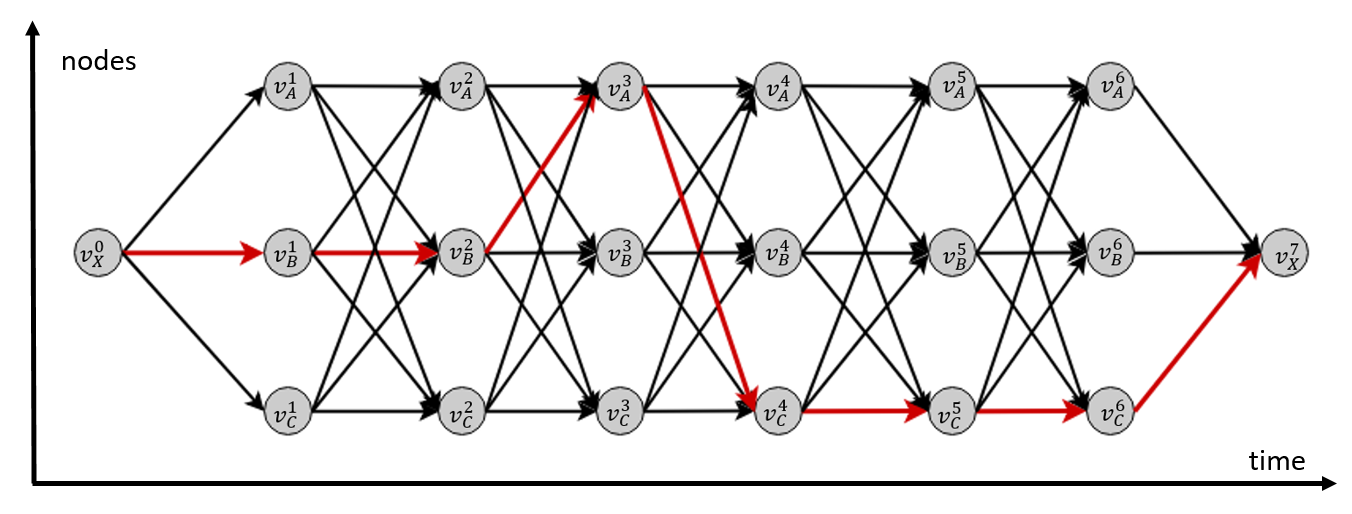
\includegraphics[width=1.0\columnwidth]{./imgs/multipartite_axis.png}
  \caption{Illustration of a Flying Tourist Problem using a multipartite graph. To each node (A,B,C) it is associated a waiting period of respectively (1,2,3) time units. The red arrows represent a possible solution to the problem.}
  \label{fig:multipartite_sol}  
\end{figure}


Despite the apparent complexity of the proposed definition, it can be used to
state very simple flight searches, including one-way and round-trip flights. For
example, the problem of finding a single flight from $A$ to $B$ at date $T$ can
be instantiated as a FTP given by $v_0$ = $A$, $v_{n+1}$ = $B$, $T_{0} = T$, and
$V$ = $D$ = $TW$ = $\{\}$. In its turn, a round-trop flight involving the same
two cities and the same start date, in which the staying period in $B$ is $b$
days, is given by $v_0 = v_{n+1} = A$, $T_{0} = X$, $V = \{B\}$, $D = \{b\}$ and
$TW$ = $\{\}$. Thus, this definition is adequate either for simple and complex
trips, which can be customized according to the user search criteria, by setting
either an extended start dates, or flexible duratopm.

%%______________________________________________________________
%%_____________________ Relation to TSP ________________________
%%______________________________________________________________
\subsection{Relation to the TSP}

As previously stated, the proposed FTP is closely related to the TSP and to its
time-dependent variation. Given the following list of constraints:

\todo{Explain each of these constraints}
\todo{Make item spacing smaller}

\begin{enumerate}
      \item $v_{n+1} = v_0$;
      \item $T_0 = 0$;
      \item $TW(i) = [0, +\infty[$, $\forall i \in V$;
      \item $D(i) = 1$, $\forall i \in V$;
    \item $c_{ij}^{t} = c_{ij}$, $\forall i, j \in V$, $\forall t$.
\end{enumerate}
constraints (1-4) enable the reduction of the devised FTP to a TDTSP, as
proposed by J.C.Picard (\cite{tdtsp_picard}), and the final constraint (5)
reduces the problem to the classical TSP.

Since the FTP occurs as a generalization of the TSP, and given that the latter
problem is well-known to be Np-hard complex, than so is the former one.
\todo{Insert NP-hard reference here}



%%______________________________________________________________
%%_____________________ Graph construction _____________________
%%______________________________________________________________
\subsection{Graph construction}
\label{sec:graph}

\todo{Simplify things. Remove the excess and vaguenes. Try something like this. Define a start node. 2) Schedule a date. 3) Decide where to fly to. 4) Get the possible flights. 5) Decide which are best.}
By considering the presented FTP definition, the total number of layers ($k$) of
the devised multipartite graph represents the total time span between the
earliest date at which the trip might start and the latest date in which it
should finish. The arcs that connect those nodes are divided into three groups:
\textit{initial}, \textit{transition} and \textit{final} arcs.

The \textit{initial} arcs are those which might initiate the trip. Consequently,
they must start at node $v_0$, at a time $t \in T_0 = [T_{0m}, T_{0M}]$,
connecting $v_0$ to every node in $V$. There are a total of $k_i = T_{0M} -
T_{0m} + 1$ layers for the initial arcs.

Conversely, the \textit{final} arcs are those that connect every node in $V$ to
the return node, $v_{n+1}$. There are as many final layers as there are initial
layers, and the final layer extends from $T_{fm}$ to $T_{fM}$, where $T_{fm}$ =
$T_{0m} + \sum(D)$ and $T_{fM}$ = $T_{0M} + \sum(D)$, where $\sum(D)$
corresponds to the summation of all entries belonging to $D$. In the example
depicted in Figure~\ref{fig:multipartite_sol}, there is a single initial and
final layer, since there is only one possible start date.

The \textit{transition} arcs are those which fully connect the $N$ nodes
belonging to $V$. The earliest transition arc occurs at a time no sooner than
$t_1 = T_{0m} + min(D)$, where $min(D)$ corresponds to the lowest entry of the
set of staying durations. Hence, if the trip starts by transiting an initial arc
at time $T_{0m}$, the first transition arc might only be traversed $min(D)$
time-units later. By following a similar approach, the latest transition arc can
occur no latter than $t_2 = T_{0M} + \sum(D) - min(D)$. Thus, there are a total
of $k_2 = t_2-t_1+1$ transition layers, and $k_2*n*(n-1)$ transition arcs.

The union of the initial, transition and final arcs gives the set $A$ of all the
arcs, which may be used to construct a solution to the requested trip. 

Having the information relative to the multipartite graph associated to the
devised FTP, it is now possible to construct a three-dimensional array matrix
representing this problem, where each entry of the array corresponds to an arc
connecting two nodes, at a particular moment in time. This weight matrix is
initialized with a very high cost value (as to reject arcs which may not be part
of the solution), and every entry of it is updated according to the information
of the multipartite graph and the respective objective function. Finally, this
weight matrix may be used as input for the optimization system (see
section
\todo{Insert reference}).
%~\ref{sec:optimization}).

Although it is clear that any arc $a \in A$ corresponds to a particular flight,
it should be noted that no specific or limiting assumption was considered up
until now. Instead, it was assumed an entirely abstract arc definition,
connecting two nodes at a specific moment in time. In order to transform this
set of arcs into a corresponding set of flights, it is necessary to obtain
real-world flight data from some external source. This will be further detailed
in section
\todo{Insert reference}
%~\ref{sec:system}.












% If Printing on DOUBLE SIDED pages, the second page should be white.
% Otherwise, comment the following command:
\cleardoublepage


%% _____________________ TEST 
%% _____________________ TEST 
i added some text here
%% _____________________ TEST 


%
% -----------------------------------------------------------------------------




















% BIBLIOGRAPHY
% Add the Bibliography to the PDF table of contents (not the document table of contents)
\pdfbookmark[0]{Bibliography}{bib}
% The bibliography style sheet
% Chose your preferences on the format of the entries and the Labels:
% IEEEtran: Used in general (recommended for IST Thesis)
%           Entries are labelled and sorted by appearance in the document
%           Labels are Numeric inside square brackets
\bibliographystyle{IEEEtran}
%
% Apalike:  Entries formatted alphabetically, last name first, with identation
%           Labels with Autor's Name and Year inside square brackets
%\bibliographystyle{apalike}
%
% Alpha:    Entries formatted with Autor's Name and Year, hanging identation
%           Labels with Autor's abbr. Names and Year inside square brackets
%\bibliographystyle{alpha}
%
% Acm:     Entries formatted with Autor's Name (small Caps), hanging identation
%          Labels are Numeric inside square brackets
%\bibliographystyle{acm}
% The following command resets the 'emphasis' style for bibliography entries
\normalem
% Name of your BiBTeX file
\bibliography{./Thesis-MSc-Bibliography} % Put here your own filename
%
% The following command modifies the 'emphasis' style for bibliography entries
\ULforem
% If Printing on DOUBLE SIDED pages, the second page should be white.
% Otherwise, comment the following command:
\cleardoublepage
%
% -----------------------------------------------------------------------------
% HERE GO THE APPENDIXES IF REQUIRED
% If not required just comment the blocks
\appendix
%% First Appendix
\pdfbookmark[1]{Appendix A}{appendix}
% #############################################################################
% This is Appendix A
% !TEX root = ../main.tex
% #############################################################################
\chapter{Code of Project}
\label{chapter:appendixA}

Nulla dui purus, eleifend vel, consequat non, dictum porta, nulla. Duis ante mi, laoreet ut, commodo eleifend, cursus nec, lorem. Aenean eu est. Etiam imperdiet turpis. Praesent nec augue. Curabitur ligula quam, rutrum id, tempor sed, consequat ac, dui. Vestibulum accumsan eros nec magna. Vestibulum vitae dui. Vestibulum nec ligula et lorem consequat ullamcorper. 

\begin{lstlisting}[frame=lines,style=XML,caption={Example of a XML file.},label=xmlEx]
<?xml version="1.0" encoding="UTF-8"?>
<StreamInfo version="2.0">
    <Clip duration="PT01M0.00S">
        <BaseURL>videos/</BaseURL>
        <Description>svc_1</Description>
        <Representation mimeType="video/SVC" codecs="svc" frameRate="30.00" bandwidth="401.90"
            width="176" height="144" id="L0">
            <BaseURL>svc_1/</BaseURL>
            <SegmentInfo from="0" to="11" duration="PT5.00S">
                <BaseURL>svc_1-L0-</BaseURL>
            </SegmentInfo>
        </Representation>
        <Representation mimeType="video/SVC" codecs="svc" frameRate="30.00" bandwidth="1322.60"
            width="352" height="288" id="L1">
            <BaseURL>svc_1/</BaseURL>
            <SegmentInfo from="0" to="11" duration="PT5.00S">
                <BaseURL>svc_1-L1-</BaseURL>
            </SegmentInfo>
        </Representation>
    </Clip>
</StreamInfo>
\end{lstlisting}

Etiam imperdiet turpis. Praesent nec augue. Curabitur ligula quam, rutrum id, tempor sed, consequat ac, dui. Maecenas tincidunt velit quis orci. Sed in dui. Nullam ut mauris eu mi mollis luctus. Class aptent taciti sociosqu ad litora torquent per conubia nostra, per inceptos hymenaeos. Sed cursus cursus velit. Sed a massa. Duis dignissim euismod quam.

\begin{spacing}{0.5}
\lstinputlisting[style=coloredASM,language=Assembler,numbers=left,caption={Assembler Main Code.},label=code]
{./tables_and_code/example.asm.txt}
\end{spacing}


Class aptent taciti sociosqu ad litora torquent per conubia nostra, per inceptos hymenaeos. Phasellus eget nisl ut elit porta ullamcorper. Maecenas tincidunt velit quis orci. Sed in dui. Nullam ut mauris eu mi mollis luctus. Class aptent taciti sociosqu ad litora torquent per conubia nostra, per inceptos hymenaeos.

This inline MATLAB code \mcode{for i=1:3, disp('cool'); end;} uses the \verb|\mcode{}| command.\footnote{MATLAB Works also in footnotes: \mcodefn{for i=1:3, disp('cool'); end;}}

Nullam ut mauris eu mi mollis luctus. Class aptent taciti sociosqu ad litora torquent per conubia nostra, per inceptos hymenaeos. Sed cursus cursus velit. Sed a massa. Duis dignissim euismod quam. Nullam euismod metus ut orci.

\begin{lstlisting}[language=matlabfloz,caption={\mcode{Matlab Function}}]
for i = 1:3
	if i >= 5 && a ~= b       % literate programming replacement
		disp('cool');         % comment with some §\mcommentfont\LaTeX in it: $\mcommentfont\pi x^2$§
	end
	[:,ind] = max(vec);
	x_last = x(1,end) - 1;
	v(end);
	ylabel('Voltage (µV)');
end
\end{lstlisting}

Nullam ut mauris eu mi mollis luctus. Class aptent taciti sociosqu ad litora torquent per conubia nostra, per inceptos hymenaeos. Sed cursus cursus velit. Sed a massa. Duis dignissim euismod quam. Nullam euismod metus ut orci.

\lstinputlisting[
	label=lst:matlab_code,
	caption={\mcode{function.m}},
	breaklines=true
	]{./tables_and_code/function.m}

Class aptent taciti sociosqu ad litora torquent per conubia nostra, per inceptos hymenaeos. Phasellus eget nisl ut elit porta ullamcorper. Maecenas tincidunt velit quis orci. Sed in dui. Nullam ut mauris eu mi mollis luctus. Class aptent taciti sociosqu ad litora torquent per conubia nostra, per inceptos hymenaeos. Sed cursus cursus velit. Sed a massa. Duis dignissim euismod quam. Nullam euismod metus ut orci. Vestibulum erat libero, scelerisque et, porttitor et, varius a, leo.

\begin{lstlisting}[style=htmlcssjs,caption={HTML with CSS Code}]
<!DOCTYPE html>
<html>
  <head>
    <title>Listings Style Test</title>
    <meta charset="UTF-8">
    <style>
      /* CSS Test */
      * {
        padding: 0;
        border: 0;
        margin: 0;
      }
    </style>
    <link rel="stylesheet" href="css/style.css" />
  </head>
  <header> hey </header>
  <article> this is a article </article>
  <body>
    <!-- Paragraphs are fine -->
    <div id="box">			
			<p>
			  Hello World
			</p>
      <p>Hello World</p>
      <p id="test">Hello World</p>
			<p></p>
    </div>
    <div>Test</div>
    <!-- HTML script is not consistent -->
    <script src="js/benchmark.js"></script>
    <script>
      function createSquare(x, y) {
        // This is a comment.
        var square = document.createElement('div');
        square.style.width = square.style.height = '50px';
        square.style.backgroundColor = 'blue';
        
        /*
         * This is another comment.
         */
        square.style.position = 'absolute';
        square.style.left = x + 'px'; 
        square.style.top = y + 'px';
        
        var body = document.getElementsByTagName('body')[0];
        body.appendChild(square);
      };
      
      // Please take a look at +=
      window.addEventListener('mousedown', function(event) {
        // German umlaut test: Berührungspunkt ermitteln
        var x = event.touches[0].pageX;
        var y = event.touches[0].pageY;
        var lookAtThis += 1;
      });
    </script>
  </body>
</html>
\end{lstlisting}

Nulla dui purus, eleifend vel, consequat non, dictum porta, nulla. Duis ante mi, laoreet ut, commodo eleifend, cursus nec, lorem. Aenean eu est. Etiam imperdiet turpis. Praesent nec augue. Curabitur ligula quam, rutrum id, tempor sed, consequat ac, dui. Vestibulum accumsan eros nec magna. Vestibulum vitae dui. Vestibulum nec ligula et lorem consequat ullamcorper.

\begin{lstlisting}[style=htmlcssjs,caption={HTML CSS Javascript Code}]

@media only screen and (min-width: 768px) and (max-width: 991px) {
	
	#main {
		width: 712px;
		padding: 100px 28px 120px;
	}
	
	/* .mono {
		font-size: 90%;
	} */
	
	.cssbtn a {
		margin-top: 10px;
		margin-bottom: 10px;
		width: 60px;  
		height: 60px;   
		font-size: 28px;
		line-height: 62px;
	}
\end{lstlisting}

Nulla dui purus, eleifend vel, consequat non, dictum porta, nulla. Duis ante mi, laoreet ut, commodo eleifend, cursus nec, lorem. Aenean eu est. Etiam imperdiet turpis. Praesent nec augue. Curabitur ligula quam, rutrum id, tempor sed, consequat ac, dui. Vestibulum accumsan eros nec magna. Vestibulum vitae dui. Vestibulum nec ligula et lorem consequat ullamcorper.

\begin{lstlisting} [style=py,caption={PYTHON Code}]
class TelgramRequestHandler(object):
    def handle(self):
        addr = self.client_address[0]         # Client IP-adress
        telgram = self.request.recv(1024)     # Recieve telgram
        print "From: %s, Received: %s" % (addr, telgram)
        return
\end{lstlisting}
%% If Printing on DOUBLE SIDED pages, the second page should be white.
%% Otherwise, comment the following command:
\cleardoublepage
%% Second Appendix
\pdfbookmark[1]{Appendix B}{appendix}
% #############################################################################
% This is Appendix B
% !TEX root = ../main.tex
% #############################################################################
\chapter{A Large Table}
\label{chapter:appendixB}

Aliquam et nisl vel ligula consectetuer suscipit. Morbi euismod enim eget neque. Donec sagittis massa. Vestibulum quis augue sit amet ipsum laoreet pretium. Nulla facilisi. Duis tincidunt, felis et luctus placerat, ipsum libero vestibulum sem, vitae elementum wisi ipsum a metus. Nulla a enim sed dui hendrerit lobortis. Donec lacinia vulputate magna. Vivamus suscipit lectus at quam. In lectus est, viverra a, ultricies ut, pulvinar vitae, tellus. Donec et lectus et sem rutrum sodales. Morbi cursus. Aliquam a odio. Sed tortor velit, convallis eget, porta interdum, convallis sed, tortor. Phasellus ac libero a lorem auctor mattis. Lorem ipsum dolor sit amet, consectetuer adipiscing elit.

Nunc auctor bibendum eros. Maecenas porta accumsan mauris. Etiam enim enim, elementum sed, bibendum quis, rhoncus non, metus. Fusce neque dolor, adipiscing sed, consectetuer et, lacinia sit amet, quam. Suspendisse wisi quam, consectetuer in, blandit sed, suscipit eu, eros. Etiam ligula enim, tempor ut, blandit nec, mollis eu, lectus. Nam cursus. Vivamus iaculis. Aenean risus purus, pharetra in, blandit quis, gravida a, turpis. Donec nisl. Aenean eget mi. Fusce mattis est id diam. Phasellus faucibus interdum sapien. Duis quis nunc. Sed enim.
Nunc auctor bibendum eros. Maecenas porta accumsan mauris. Etiam enim enim, elementum sed, bibendum quis, rhoncus non, metus. Fusce neque dolor, adipiscing sed, consectetuer et, lacinia sit amet, quam.

% Table Example
\newcommand{\greyrow}{\rowcolor[rgb]{0.9,0.9,0.9}}
\newcommand{\whiterow}{\rowcolor[rgb]{1,1,1}}
\newcommand{\greycell}[1]{\multicolumn{1}{{>{\columncolor[rgb]{0.9,0.9,0.9}}c}}{#1}}
\newcommand{\lightgreycell}[1]{\multicolumn{1}{{>{\columncolor[rgb]{0.9,0.9,0.9}}c}}{#1}}
\newcommand{\mediumgreycell}[1]{\multicolumn{1}{{>{\columncolor[rgb]{0.8,0.8,0.8}}c}}{#1}}
\newcommand{\darkgreycell}[1]{\multicolumn{1}{{>{\columncolor[rgb]{0.7,0.7,0.7}}c}}{#1}}
\newcommand{\whitecell}[1]{\multicolumn{1}{{>{\columncolor[rgb]{1,1,1}}c}}{#1}}

\newcommand{\cellformatG}[1]{\multicolumn{1}{{>{\columncolor[rgb]{.9,.9,.9}}c}}{#1}}
\newcommand{\cellformatW}[1]{\multicolumn{1}{{>{\columncolor[rgb]{1,1,1}}c}}{#1}}
\newcommand{\cellformatlG}[1]{\multicolumn{1}{{|>{\columncolor[rgb]{.9,.9,.9}}c}}{#1}}
\newcommand{\cellformatlW}[1]{\multicolumn{1}{{|>{\columncolor[rgb]{1,1,1}}c}}{#1}}
\newcommand{\cellformatrG}[1]{\multicolumn{1}{{>{\columncolor[rgb]{.9,.9,.9}}c|}}{#1}}
\newcommand{\cellformatrW}[1]{\multicolumn{1}{{>{\columncolor[rgb]{1,1,1}}c|}}{#1}}
\newcommand{\cellformatlrG}[1]{\multicolumn{1}{{|>{\columncolor[rgb]{.9,.9,.9}}c|}}{#1}}
\newcommand{\cellformatlrW}[1]{\multicolumn{1}{{|>{\columncolor[rgb]{1,1,1}}c|}}{#1}}

\begin{table}[t]
\centering
\caption{Example table}
\label{table:table1}
\begin{tabular}{c c c c c c}
\hline
\cellformatrG{}&\cellformatlG{}&\cellformatrG{}&\cellformatlG{}&\cellformatrG{}&\cellformatlG{}\\
\cellformatrG{}&
\cellformatlG{\multirow{-2}{*}{\centering\bf \#Layers}} & 
\cellformatrG{\multirow{-2}{*}{\centering\bf \#Nets}} & 
\cellformatlG{\multirow{-2}{*}{\centering \#Nodes\Mark1}} & 
\cellformatrG{\multirow{-2}{1.8cm}{\centering Critical path}}&
\cellformatlG{\multirow{-2}{2cm}{\centering\bf Latency ($T_{iter}$)}}\\
\cellformatrG{\multirow{-3}{2.2cm}{\centering Benchmark: ANN}} &
\cellformatlG{\footnotesize $(1)$} & 
\cellformatrG{\footnotesize$(2)$} & 
\cellformatlG{\footnotesize$(3)=8\cdot(1)\cdot(2)$} & 
\cellformatrG{\footnotesize$(4)=4\cdot(1)$} & 
\cellformatlG{\footnotesize$(5)$}\\
\hline
\cellformatrW{A1} & \cellformatlW{\bf 3--1501} & \cellformatrW{       1   } & \cellformatlW{\bf 24--12008}  & \cellformatrW{\bf 12--6004} & \cellformatlW{    4}\\
\cellformatrW{A2} & \cellformatlW{    501    } & \cellformatrW{       1   } & \cellformatlW{     4008    }  & \cellformatrW{  2004      } & \cellformatlW{\bf 2--2000 }\\
\cellformatrW{A3} & \cellformatlW{     10    } & \cellformatrW{\bf 2--1024} & \cellformatlW{\bf 160--81920} & \cellformatrW{    40      } & \cellformatlW{   60\Mark2 }\\
\cellformatrW{A4} & \cellformatlW{     10    } & \cellformatrW{      50   } & \cellformatlW{     4000    }  & \cellformatrW{    40      } & \cellformatlW{\bf 80--1200}\\
\hline
\multicolumn{6}{c}{\vspace*{-0.3cm}}\\
%%%%%%%%%%%%% SECOND PART OF THE TABLE %%%%%%%%%%%%%%%%%%%%%%%%
\hline
\cellformatrG{}&\cellformatlG{}&\cellformatrG{}&\cellformatlG{}&\cellformatrG{}&\cellformatlG{}\\
\cellformatrG{}&
\cellformatlG{\multirow{-2}{1.6cm}{\centering\bf FFT size\Mark3}} & 
\cellformatrG{\multirow{-2}{*}{\centering\it\#Inputs}} & 
\cellformatlG{\multirow{-2}{*}{\centering\it \#Nodes\Mark1}} & 
\cellformatrG{\multirow{-2}{1.8cm}{\centering\it Critical path}}&
\cellformatlG{\multirow{-2}{2cm}{\centering\bf Latency ($T_{iter}$)}}\\
\cellformatrG{\multirow{-3}{2.2cm}{\centering Benchmark: FFT}}& 
\cellformatlG{\footnotesize$(1)$} & 
\cellformatrG{\footnotesize$(2)=2^{(1)}$} & 
\cellformatlG{\footnotesize$(3)=10\cdot(1)\cdot (2)$} & 
\cellformatrG{\footnotesize$(4)=4\cdot (1)$} & 
\cellformatlG{\footnotesize$(5)$}\\
\hline
\cellformatrW{F1} & \cellformatlW{\bf 1--10} & \cellformatrW{2--1024} & \cellformatlW{\bf 20--102400} &  \cellformatrW{4--40} & \cellformatlW{6--60\Mark2}\\
\cellformatrW{F2} & \cellformatlW{\bf 5} & \cellformatrW{32} & \cellformatlW{1600} & \cellformatrW{20} & \cellformatlW{\bf 40 -- 1500}\\
\hline
\multicolumn{6}{c}{\vspace*{-0.3cm}}\\
% THIRD AND LAST TABLE!!!
\hline
\cellformatrG{}&\cellformatlG{}&\cellformatrG{}&\cellformatlG{}&\cellformatrG{}&\cellformatlG{}\\
\cellformatrG{}&
\cellformatlG{\multirow{-2}{*}{\centering\bf\#Types}} & 
\cellformatrG{\multirow{-2}{*}{\centering\bf \#Nodes}} & 
\cellformatlG{\multirow{-2}{*}{\centering\it \#Networks}} & 
\cellformatrG{\multirow{-2}{1.8cm}{\centering\it Critical path}}&
\cellformatlG{\multirow{-2}{2cm}{\centering\bf Latency ($T_{iter}$)}}\\
\cellformatrG{\multirow{-3}{2.2cm}{\centering Benchmark: Random networks}}& 
\cellformatlG{\footnotesize$(1)$} & 
\cellformatrG{\footnotesize$(2)$} & 
\cellformatlG{\footnotesize$(3)$} &
\cellformatrG{\footnotesize$(4)$} & 
\cellformatlG{\footnotesize$(5)$}\\
\hline
\cellformatrW{R1} & \cellformatlW{3} & \cellformatrW{10--2000} & \cellformatlW{500} &  \cellformatrW{\it variable} & \cellformatlW{\footnotesize$(4)$}\\
\cellformatrW{R2} & \cellformatlW{3} & \cellformatrW{  50    } & \cellformatlW{500} &  \cellformatrW{\it variable} & \cellformatlW{\footnotesize$(4)\times [1;\cdots;20]$}\\
\hline
\multicolumn{6}{c}{\vspace*{-0.3cm}}\\
\multicolumn{6}{l}{\it\Mark1 Excluding constant nodes.}\\
\multicolumn{6}{l}{\it\Mark2 Value kept proportional to the critical path: $(5)=(4)*1.5$.}\\
\multicolumn{6}{l}{\it\Mark3 A size of $x$ corresponds to a $2^x$ point FFT.}\\
\multicolumn{6}{l}{\it Values in bold indicate the parameter being varied.}
\end{tabular}
\end{table}

\textcolor{violet}{As \Cref{table:table1} shows, the data can be inserted from a file, in the case of a somehow complex structure. Notice the Table footnotes.}	

Lorem ipsum dolor sit amet, consectetuer adipiscing elit. Morbi commodo, ipsum sed pharetra gravida, orci magna rhoncus neque, id pulvinar odio lorem non turpis. Nullam sit amet enim. Suspendisse id velit vitae ligula volutpat condimentum. Aliquam erat volutpat. Sed quis velit. Nulla facilisi. Nulla libero. Vivamus pharetra posuere sapien. Nam consectetuer. Sed aliquam, nunc eget euismod ullamcorper, lectus nunc ullamcorper orci, fermentum bibendum enim nibh eget ipsum. Donec porttitor ligula eu dolor. Maecenas vitae nulla consequat libero cursus venenatis. Nam magna enim, accumsan eu, blandit sed, blandit a, eros. 

\textcolor{violet}{And now an example (\Cref{tab:lon_table}) of a table that extends to more than one page. Notice the repetition of the Caption (with indication that is continued) and of the Header, as well as the continuation text at the bottom.}

\begin{center}
\begin{longtable}{|l|l|l|}
\caption[Example of a very long table spreading in several pages]{Example of a very long table spreading in several pages} \label{tab:lon_table} \\

\hline \multicolumn{1}{|c|}{\textbf{Time (s)}} & \multicolumn{1}{c|}{\textbf{Triple chosen}} & \multicolumn{1}{c|}{\textbf{Other feasible triples}} \\ \hline 
\endfirsthead

\multicolumn{3}{c}%
{{\bfseries \tablename\ \thetable{} -- continued from previous page}} \\
\hline \multicolumn{1}{|c|}{\textbf{Time (s)}} &
\multicolumn{1}{c|}{\textbf{Triple chosen}} &
\multicolumn{1}{c|}{\textbf{Other feasible triples}} \\ \hline 
\endhead

\hline \multicolumn{3}{|r|}{{Continued on next page}} \\ \hline
\endfoot

\hline \hline
\endlastfoot
0 & (1, 11, 13725) & (1, 12, 10980), (1, 13, 8235), (2, 2, 0), (3, 1, 0) \\
2745 & (1, 12, 10980) & (1, 13, 8235), (2, 2, 0), (2, 3, 0), (3, 1, 0) \\
5490 & (1, 12, 13725) & (2, 2, 2745), (2, 3, 0), (3, 1, 0) \\
8235 & (1, 12, 16470) & (1, 13, 13725), (2, 2, 2745), (2, 3, 0), (3, 1, 0) \\
10980 & (1, 12, 16470) & (1, 13, 13725), (2, 2, 2745), (2, 3, 0), (3, 1, 0) \\
13725 & (1, 12, 16470) & (1, 13, 13725), (2, 2, 2745), (2, 3, 0), (3, 1, 0) \\
16470 & (1, 13, 16470) & (2, 2, 2745), (2, 3, 0), (3, 1, 0) \\
19215 & (1, 12, 16470) & (1, 13, 13725), (2, 2, 2745), (2, 3, 0), (3, 1, 0) \\
21960 & (1, 12, 16470) & (1, 13, 13725), (2, 2, 2745), (2, 3, 0), (3, 1, 0) \\
24705 & (1, 12, 16470) & (1, 13, 13725), (2, 2, 2745), (2, 3, 0), (3, 1, 0) \\
27450 & (1, 12, 16470) & (1, 13, 13725), (2, 2, 2745), (2, 3, 0), (3, 1, 0) \\
30195 & (2, 2, 2745) & (2, 3, 0), (3, 1, 0) \\
32940 & (1, 13, 16470) & (2, 2, 2745), (2, 3, 0), (3, 1, 0) \\
35685 & (1, 13, 13725) & (2, 2, 2745), (2, 3, 0), (3, 1, 0) \\
38430 & (1, 13, 10980) & (2, 2, 2745), (2, 3, 0), (3, 1, 0) \\
41175 & (1, 12, 13725) & (1, 13, 10980), (2, 2, 2745), (2, 3, 0), (3, 1, 0) \\
43920 & (1, 13, 10980) & (2, 2, 2745), (2, 3, 0), (3, 1, 0) \\
46665 & (2, 2, 2745) & (2, 3, 0), (3, 1, 0) \\
49410 & (2, 2, 2745) & (2, 3, 0), (3, 1, 0) \\
52155 & (1, 12, 16470) & (1, 13, 13725), (2, 2, 2745), (2, 3, 0), (3, 1, 0) \\
54900 & (1, 13, 13725) & (2, 2, 2745), (2, 3, 0), (3, 1, 0) \\
57645 & (1, 13, 13725) & (2, 2, 2745), (2, 3, 0), (3, 1, 0) \\
60390 & (1, 12, 13725) & (2, 2, 2745), (2, 3, 0), (3, 1, 0) \\
63135 & (1, 13, 16470) & (2, 2, 2745), (2, 3, 0), (3, 1, 0) \\
65880 & (1, 13, 16470) & (2, 2, 2745), (2, 3, 0), (3, 1, 0) \\
68625 & (2, 2, 2745) & (2, 3, 0), (3, 1, 0) \\
71370 & (1, 13, 13725) & (2, 2, 2745), (2, 3, 0), (3, 1, 0) \\
74115 & (1, 12, 13725) & (2, 2, 2745), (2, 3, 0), (3, 1, 0) \\
76860 & (1, 13, 13725) & (2, 2, 2745), (2, 3, 0), (3, 1, 0) \\
79605 & (1, 13, 13725) & (2, 2, 2745), (2, 3, 0), (3, 1, 0) \\
82350 & (1, 12, 13725) & (2, 2, 2745), (2, 3, 0), (3, 1, 0) \\
85095 & (1, 12, 13725) & (1, 13, 10980), (2, 2, 2745), (2, 3, 0), (3, 1, 0) \\
87840 & (1, 13, 16470) & (2, 2, 2745), (2, 3, 0), (3, 1, 0) \\
90585 & (1, 13, 16470) & (2, 2, 2745), (2, 3, 0), (3, 1, 0) \\
93330 & (1, 13, 13725) & (2, 2, 2745), (2, 3, 0), (3, 1, 0) \\
96075 & (1, 13, 16470) & (2, 2, 2745), (2, 3, 0), (3, 1, 0) \\
98820 & (1, 13, 16470) & (2, 2, 2745), (2, 3, 0), (3, 1, 0) \\
101565 & (1, 13, 13725) & (2, 2, 2745), (2, 3, 0), (3, 1, 0) \\
104310 & (1, 13, 16470) & (2, 2, 2745), (2, 3, 0), (3, 1, 0) \\
107055 & (1, 13, 13725) & (2, 2, 2745), (2, 3, 0), (3, 1, 0) \\
109800 & (1, 13, 13725) & (2, 2, 2745), (2, 3, 0), (3, 1, 0) \\
112545 & (1, 12, 16470) & (1, 13, 13725), (2, 2, 2745), (2, 3, 0), (3, 1, 0) \\
115290 & (1, 13, 16470) & (2, 2, 2745), (2, 3, 0), (3, 1, 0) \\
118035 & (1, 13, 13725) & (2, 2, 2745), (2, 3, 0), (3, 1, 0) \\
120780 & (1, 13, 16470) & (2, 2, 2745), (2, 3, 0), (3, 1, 0) \\
123525 & (1, 13, 13725) & (2, 2, 2745), (2, 3, 0), (3, 1, 0) \\
126270 & (1, 12, 16470) & (1, 13, 13725), (2, 2, 2745), (2, 3, 0), (3, 1, 0) \\
129015 & (2, 2, 2745) & (2, 3, 0), (3, 1, 0) \\
131760 & (2, 2, 2745) & (2, 3, 0), (3, 1, 0) \\
134505 & (1, 13, 16470) & (2, 2, 2745), (2, 3, 0), (3, 1, 0) \\
137250 & (1, 13, 13725) & (2, 2, 2745), (2, 3, 0), (3, 1, 0) \\
139995 & (2, 2, 2745) & (2, 3, 0), (3, 1, 0) \\
142740 & (2, 2, 2745) & (2, 3, 0), (3, 1, 0) \\
145485 & (1, 12, 16470) & (1, 13, 13725), (2, 2, 2745), (2, 3, 0), (3, 1, 0) \\
148230 & (2, 2, 2745) & (2, 3, 0), (3, 1, 0) \\
150975 & (1, 13, 16470) & (2, 2, 2745), (2, 3, 0), (3, 1, 0) \\
153720 & (1, 12, 13725) & (2, 2, 2745), (2, 3, 0), (3, 1, 0) \\
156465 & (1, 13, 13725) & (2, 2, 2745), (2, 3, 0), (3, 1, 0) \\
159210 & (1, 13, 13725) & (2, 2, 2745), (2, 3, 0), (3, 1, 0) \\
161955 & (1, 13, 16470) & (2, 2, 2745), (2, 3, 0), (3, 1, 0) \\
164700 & (1, 13, 13725) & (2, 2, 2745), (2, 3, 0), (3, 1, 0) \\
\end{longtable}
\end{center}
%% If Printing on DOUBLE SIDED pages, the second page should be white.
%% Otherwise, comment the following command:
\cleardoublepage

% -----------------------------------------------------------------------------
% And this is THE END of the IST Thesis Document
\end{document}